\documentclass[12pt,oneside,a4paper]{article}

\usepackage{./top/custom}

\usepackage[backend=biber]{biblatex}
\addbibresource{./top/biblio.bib}
\setcounter{tocdepth}{2}

\lstset{language=Julia}

% new commands (fold)
\newcounter{nalg}[section] % defines algorithm counter for chapter-level
\renewcommand{\thenalg}{\thechapter .\arabic{nalg}} %defines appearance of the algorithm counter
\DeclareCaptionLabelFormat{algocaption}{Algorithm \thenalg} % defines a new caption label as Algorithm x.y

\lstnewenvironment{algorithm}[1][] %defines the algorithm listing environment
{   
    \lstset{ %this is the stype
        frame=tB,
        numbers=left, 
        numberstyle=\tiny,
        basicstyle=\scriptsize, 
        keywordstyle=\color{black}\bfseries\em,
        keywords={,input, output, return, datatype, function, in, if, else, foreach, while, begin, end, } %add the keywords you want, or load a language as Rubens explains in his comment above.
        numbers=left,
        xleftmargin=.04\textwidth,
        #1 % this is to add specific settings to an usage of this environment (for instnce, the caption and referable label)
    }
    \refstepcounter{nalg} %increments algorithm number
    \captionsetup{labelformat=algocaption,labelsep=colon} %defines the caption setup for: it ises label format as the declared caption label above and makes label and caption text to be separated by a ':'
}
{}

\usepackage{algorithm}% http://ctan.org/pkg/algorithms
\usepackage{algpseudocode}% http://ctan.org/pkg/algorithmicx
\newcommand{\var}[1]{{\ttfamily#1}}% variable

% new commands (end)

\begin{document}
\begin{titlepage}
\begin{center}

%
\includegraphics[scale=0.5]{./img/logo_centralesup.jpg} \hfill
%
\includegraphics[scale=0.3]{./img/logo_digiplante.png}

\vfill 

\textsc{\Large Projet enjeu : Santé et biotechnologies}\\[0.5cm]

\vfill

\textsc{\Large Rapport final}\\[1.5cm] 

% Title
\HRule \\[0.4cm]
{ \LARGE \bfseries Développement d'outils mathématiques \\ 
   pour l'agriculture de précision \\[0.4cm] }

\HRule \\[1.5cm]

\vfill

{\large
\begin{center}
  \textbf{Client et Référent Pédagogique} \\~\\
\begin{tabular}{rl}
   \quad Pierre &\textsc{Carmier} \\
    \quad Paul-Henry &\textsc{Courn\`ede} \\
  
\end{tabular}
\end{center}
\vfill
\begin{center}
  \textbf{P2018 : groupe SBT-11} \\~\\
  
\begin{tabular}{rl}

    \quad John &\textsc{de Wasseige} \\
    \quad Nayef &\textsc{Derwiche} \\
    \quad Alexis &\textsc{Mathey} \\
    \quad Daina &\textsc{Zheng} \\ \\
\end{tabular}
\end{center}
}

\vfill

{\large 10 juin 2015}

\end{center}
\end{titlepage}

{\hypersetup{linkcolor=black}
\tableofcontents
}
\newpage

\section*{Résumé}
\addcontentsline{toc}{section}{Résumé}
Ce rapport présente nos résultats et nos perspectives
du projet et s'articule autour de cinq parties.

Dans un premier temps, nous introduisons le contexte global du
projet en mettant l'accent sur l'objectif poursuivi par celui-ci.

On expose ensuite une synthèse de l'\emph{étude documentaire}
en décrivant brièvement chacun des thèmes abordés dans celle-ci.
On rappelera notamment quelques notions de physiologie des plantes, un bref historique de la modélisation des plantes
ainsi que les principaux modèles actuels et leurs caractéristiques communes.

La partie suivante décrit l'ensemble des méthodes
utilisées pour mener à bien notre projet.
On décrira d'abord les outils de travail que nous avons
utilisés afin de collaborer efficacement.
On rappelera ensuite la façon dont nous avons
géré notre bibliographie.
Un planning de la répartition des tâches à travers
le semestre sera ensuite donné.
On terminera cette partie en décrivant de façon
exhaustive les difficultés que nous avons rencontrées
jusqu'à maintenant.

Avant de décrire les résultats obtenus,
nous rappelerons de manière synthétique le fonctionnement
de notre modèle.
On expliquera ensuite comment nous avons implémenté
celui-ci en \textsc{Julia} en détaillant les
variables et fonctions utilisées.

La dernière partie reprendra d'une part nos résultats
ainsi qu'une analyse de ceux-ci et de leur pertinence
par rapport à ce que l'on observe expérimentalement,
et d'autre part les perspectives à long terme
que nous proposons pour le projet.

\newpage
\section{Introduction}


Au cours de ce projet, nous nous sommes intéressés au \emph{développement d'outils mathématiques 
pour l'agriculture de précision} en collaboration avec le laboratoire MAS (Mathématiques et Informatique pour la Complexité et les Systèmes).

Dans le contexte environnemental actuel, et alors que 2 milliards de personnes sont en sous-nutrition dans le monde, la modélisation de la croissance des plantes prend tout son sens.

En effet, le problème des ressources \textit{énergétiques} et \textit{alimentaires} est un sujet crucial du  21ème siècle.
Il faudra être capable de nourrir plus de 
9 milliards d'humains en 2050~\cite{wiki:popu_mondiale}.
De plus, les ressources fossiles et l'eau douce viennent à manquer dans de nombreuses régions agricoles (comme en Californie). Cependant, l'agriculture nécessite un apport d'eau important et consomme beaucoup d'énergie. L'agriculture est ainsi responsable de l'émission de près de 20\% des gaz à effet de serre tous les ans~\cite{GES}.

Les progrès de l'informatique et des mathématiques permettent néanmoins d'espérer une amélioration nette des rendements. L'objectif final est clair : nourrir plus de monde, en minimisant l'utilisation de pesticides, d'engrais et d'eau, et donc limiter l'impact environnemental et le réchauffement climatique. En effet, les capteurs, les satellites, les drones... permettent de collecter des données de plus en plus précises. Dans un futur proche, des modèles de plus en plus efficaces permettront sans doute de tirer parti de ses données pour améliorer considérablement les rendements.  

L'objectif premier de notre projet était d'implémenter un modèle , le modèle LNAS appliqué au blé, sur la plateforme PyGMAlion-Julia du laboratoire Digiplante. Cette implémentation constituait pour ainsi dire le livrable qui était attendu par notre client Pierre Carmier.
Une fois implémenté, nous avons pu utiliser ce modèle pour simuler les caractéristiques d'un champ de blé. Par exemple, le modèle permet d'obtenir l'évolution de la biomasse des grains de blé (quantité d'intérêt) dans le champ.

Notre client Pierre Carmier, ainsi que notre référent pédagogique Paul-Henry Cournède sont des chercheurs au laboratoire MAS
Ce laboratoire travaille notamment sur les modèles mathématiques de
croissance des plantes, en collaboration avec la startup Digiplante.

A terme, nous devrions également réaliser une analyse de sensiblité qui permettrait de quantifier l'influence des paramètres qui interviennent dans le modèle. Nous avons aussi en projet de modifier quelques aspects du modèle, en rajoutant des phénomènes comme la diffusion de l'eau dans le sol.
\newpage
\section{Synthèse de l'étude documentaire}
Cette partie se présente comme une synthèse de l’analyse bibliographique que nous avions réalisée en décembre.
Le lecteur intéressé trouvera une description plus détaillée des paragraphes suivants
dans les annexes~\ref{ann:physiologie},~\ref{ann:histoire},~\ref{ann:caracteristique}
et~\ref{ann:modele}.

Nous nous étions d’abord intéressés à la \emph{physiologie} de la plante. Cela nous a permis d’appréhender les éléments essentiels à son développement.
L’élément crucial qui permet le développement d’une plante est la \emph{photosynthèse}. En effet, la plante possède cette capacité extraordinaire de synthétiser de la matière organique à partir de matière minérale. 
Parce qu’ils interviennent dans la réaction de photosynthèse, l’eau, le soleil\dots ~sont des éléments clés de la modélisation du développement d’une plante.

Grâce à l’\emph{histoire} de l’étude des plantes, nous avons également pu comprendre le contexte dans lequel la modélisation des plantes s’inscrit aujourd’hui. C’est l’essor des mathématiques et de l’informatique qui permet d’envisager demain une modélisation efficace, avec des applications comme l’agriculture de précision. 
En effet, les mathématiques ont peu à peu formalisé la connaissance des plantes pour obtenir des modélisations plus précises.
On rappelera que la production de biomasse $Q$ est proportionnelle
\begin{enumerate}
  \item au LAI, pour Leaf Area Index, qui correspond au ratio entre la surface totale supérieure des feuilles
  vertes et la surface de sol sur laquelle se développe la culture,
  \item au PAR, pour Photosynthetically Active Radiation, qui correspond à l'énergie utile de la lumière incidente,
  \item à I, la lumière interceptée, donnée par
  \[ I = 1-e^{-k\cdot\mathrm{LAI}} \]
  \item au LUE, pour Light Use Efficiency, qui est le facteur d'efficience énergétique.
\end{enumerate}
selon
\[ 
  Q = \mathrm{LUE}\times\mathrm{PAR}\times I 
\]
On rappelera également le concept de \emph{temps thermique} qui correspond à l'accumulation de températures dépassant un certain seuil :
\[
\tau^{(n+1)} = \tau^{(n)} + \max[0, \underline{T^{(n)}} - T_c], 
\]
où $\underline{T^{(n)}}$ est l'écart de température constaté et 
$T_c$ est le seuil de variation de température qu'on impose.

Nous nous étions également intéressés aux \emph{caractéristiques} propres à la modélisation des plantes, afin de comprendre les principales difficultés qui empêchent une utilisation globale des modèles de croissance des plantes. Parmi eux, on peut citer : l’estimation difficile des paramètres d’un modèle, des techniques sophistiquées en informatique et en mathématique sont nécessaires et une diversité importante sans benchmarking des modèles ne permet pas de choisir facilement celui qui sera le plus adapté. 

% Nous nous sommes ensuite intéressés aux \emph{modèles les plus répandus} pour décrire le développement de la plante. Parmi eux, la grammaire L-système, le modèle GreenLab et le modèle LNAS appliqué à la betterave. La description fournie par les L-systèmes étant trop précise, ils conduisent à des temps de calcul trop importants et il est difficile d’estimer les nombreux paramètres qui interviennent.
% Le modèle GreenLab introduit une alternative intéressante : plutôt que de décrire l’architecture individuelle au niveau d’un champ, les organes (les feuilles, les grains…) sont remplacés par des pools de biomasse. On ne s’intéresse plus qu’à la masse totale des feuilles, des grains, des tiges… sur un champ. Un pool de biomasse commun permet de décrire la biomasse obtenue grâce à la photosynthèse. L’enjeu est maintenant de pouvoir décrire comment la biomasse sera répartie entre les différents organes de la plante à un instant $t$. Le modèle LNAS appliqué à la betterave nous a ainsi permis de nous familiariser avec un premier modèle de manière plus concrète, grâce aux formules d’allocation de biomasse de ce modèle.
% 
\newpage
\section{Méthodologies}
Nous présenterons dans cette section l'organisation générale du groupe et les outils qui nous aidé tout au long de ce projet.
On abordera d'abord les outils que nous avons utilisés pour partager 
notre travail le plus efficacement possible.
On présentera ensuite notre manière de gérer la bibliographie
ainsi que les logiciels utilisés pour ne pas perdre les sources visitées.
On détaillera ensuite l'organisation interne du groupe,
plus précisemment le système mis en place pour optimiser la communication
ainsi que la manière dont les tâches ont été réparties tout au long de ce projet.
On décrira finalement les problèmes, difficultés qui
!!!!SONT SURVENUS PARTIE A FAIRE QUAND CODE MARCHERA


\subsection{Outils de travail collaboratif}
Pour des raisons pratiques et esthétiques, nous avons décidé d'écrire
nos rapports en \LaTeX{}.
Il s'agissait donc de trouver la meilleure façon de partager le code source
et de pouvoir contrôler les changements apportés au document.
Une première idée pourrait être d'utiliser ShareLaTeX qui propose une plate-forme
de compilation en ligne ainsi qu'un système de gestion de versions
assez simple à utiliser.
Nous n'avons pas choisi cette solution notamment pour les raisons suivantes.
L'utilisateur doit être connecté dès qu'il veut travailler sur le projet,
le système de compilation est assez lent et l'utilisateur n'est pas libre
d'utiliser son éditeur de texte ou son visualisateur de \textsc{pdf} favori.

Pour palier aux problèmes décrits ci-dessus, le logiciel \texttt{git}
associé à GitHub est une très bonne alternative.
Il permet en effet à chaque membre du groupe de travailler sans être connecté
ainsi que d'utiliser son éditeur et compilateur favori.
Chaque membre travaille donc de son côté en faisant des \emph{commits}
et lorsqu'il juge que son travail est utile pour les autres, 
il \emph{push} sur le serveur.
L'algorithme du fusion, \emph{merge}, permet également de fusionner intelligemment
les lignes d'un fichier qui ont été modifiées par plusieurs membres.
Le dernier point à souligner est que \texttt{git} permet une gestion des branches,
particulièrement pratique lorsqu'on veut développer une partie du projet
sans risquer de créer des erreurs dans le programme principal.

Nous combinons donc ces deux outils pour 
\begin{enumerate}
  \item implémenter le modèle LNAS blé dans la plateforme
  Pygmalion en \textsc{Julia} %(une description plus détaillée de
%  l'objectif attendu pour cette partie est décrite dans la
%  section~\ref{sec:contexte} à la page~\pageref{sec:contexte})
  pour le client dont le code source est sur la plateforme GitLab,
  \item rédiger l'étude documentaire en partageant le code \LaTeX{}
  à l'aide d'un dossier sur 
  GitHub\footnote{\url{https://github.com/jdewasseige/projet-sbt11}}.
\end{enumerate}


\subsection{Gestion de la bibliographie}
Pour la gestion de la bibliographie au sein du document,
nous utilisons le package \texttt{biblatex}.
Celui-ci permet d'écrire l'ensemble de nos références dans un fichier \texttt{.bib}
sous la forme suivante.
\begin{verbatim}
  @online{histoire_mod_plantes,
    title = {Une histoire de la modélisation des plantes},
    author = {Philippe de Reffye and Marc Jaeger 
    and Paul-Henry Cournède},
    url = {https://interstices.info/jcms/c_38032/une-histoire-de-
    la-modelisation-des-plantes},
    year = {2009},
    month = "04",
  }
\end{verbatim}
La mise en page est alors automatique en fonction des informations fournies
et le rendu de l'exemple est présenté ci dessous.
\begin{figure}[h]
  
\includegraphics[scale=0.6]{./img/rendu_elem_bib.jpg}
\end{figure}

Cela parait à priori assez lourd d'écrire soi-même toutes les informations
en suivant cette syntaxe mais il existe des logiciels comme Zotero
qui font le travail à notre place.
Les sources trouvées sur Google Scholar peuvent également être exportées
aisément au format \texttt{BibTex}.

\subsection{Organisation et partage des tâches}
Il nous reste un dernier point à décrire, celui de la \emph{communication}
au sein du groupe.
Nous utilisons Slack\footnote{\url{https://slack.com/}} qui est un logiciel
de plus en plus utilisé pour les travaux de groupe ainsi que dans les start-ups.
Il permet d'éviter de devoir alterner entre plusieurs applications comme les mails,
DropBox et Twitter, puisqu'il permet d'être connecté
à celles-ci au sein de l'application.
On peut également créer plusieurs \emph{channels} pour séparer la communication
entre les différentes tâches.
Par exemple dans ce projet nous avons les \emph{channels} suivantes :
\texttt{general}, \texttt{etude-documentaire}, 
\texttt{planning} et \texttt{dev\_plate-forme}.
On trouve aussi un système d'historique et de gestion de fichiers efficace.

L'ensemble des tâches ainsi que leur répartition pendant l'année
est associé au planning \textsc{Gantt} qui se trouve
dans l'Annexe~\ref{ann:planning} à la page~\pageref{ann:planning}.

\subsection{Agenda}

Nos travaux au cours de ce semestre sont présentés dans ce tableau.

IMPOSSIBLE DE METTRE LA PHOTO

%\begin{figure}[h]
%	\begin{center}
%  \includegraphics[scale=0.51]{./planning.png}
%  \caption{Agenda de nos travaux au cours du second semestre.}
%  \label{fig:agenda}
%	\end{center}
%\end{figure}

\subsection{Difficultés rencontrées}

Au cours de ce projet, nous avons été confrontés à de nombreuses difficultés.

\subsubsection{Difficultés de gestion du temps}



Le temps fût une difficulté récurrente. Nous n'étions sans doute pas prêt à gérer de nous-même notre temps. C'est ainsi que nous avons réalisé l'opportunité que constitue ce type de projet. 
Jusqu'à maintenant, nous avions été confrontés la plupart du temps à des questions précises dans des examens, dont l'emploi du temps nous est imposé à l'avance. 
Ici, nous devions de nous même organiser notre temps. 
Nous pourrions nous dédouaner en soulignant l'emploi du temps chargé de nos études à Centrale. 
Mais ce projet est là pour nous rappeler qu'une organisation préalable et une répartition efficace des tâches doivent permettre d'éviter de subir le temps. Et cela s'apprend grâce à des projets comme celui-ci.

\subsubsection{Difficultés informatiques}

Nous avons également été confronté à des problèmes informatiques lors de l'implémentation et de l'utilisation du modèle.
\begin{itemize}
	\item Un bogue a empéché au début de nos premières tentatives le lancement de nos programmes. En effet, les chercheurs
du laboratoire MAS qui ont développé la plateforme utilisait les fonctions directement sur leur répertoire, alors que nous y accédions depuis le dossier principal. Il y avait un problème de chemin relatif. Il a donc fallu détecter l'origine de ce bogue avant de pouvoir commencer à utiliser nos programmes. 
	
	\item De plus, des erreurs classiques sur notre implémentation empêchaient également le bon déroulement de nos utilisations du modèle : coquilles, oublis, fautes de frappe... L'impossibilité d'utiliser la simulation à cause du bogue précédemment décrit a rendu leur détection plus ardue.

\end{itemize}
\subsubsection{Difficultés théoriques}
Enfin, le modèle directement implémenté à l'aide du document qui contenait les formules théoriques du modèle, et que nous avons implémenté, conduisait à des valeurs qui n'étaient pas cohérentes. Les connaissances de Pierre Carmier sur les modèles de croissance des plantes nous ont permis de savoir ce qui était cohérent dans nos résultats et ce qui ne l'était pas. 
Nous avons donc avec l'aide de notre client ajusté les formules que nous utilisions :  
\begin{itemize}
	\item Dans un premier temps, la croissance de la plante était trop faible. Il a fallu changer les fonctions log-normales dans les fonctions d'allocation, de remobilisation et de sénescence. 
La formule donnée dans le document  utilisait une définition différente de l'écart type que la formule qui correspondait aux paramètres que Pierre Carmier nous avait fournis. Nous avons donc utilisé directement la formule déjà implémenté dans le modèle LNAS betterave qui correspond bien aux conventions utilisées.
	\item Une fois ceci corrigé, nous obtenions cette fois des récoltes beaucoup trop élevées, plus de 3000 en grains et environ 16 de LAI, alors que les valeurs attendues sont respectivement en ordre de grandeur 1000 et entre 5 et 6.
Cela était dû à l'absence de prise en compte dans le modèle théorique du temps de montaison, temps à partir duquel la tige commence à croître de manière très rapide.

En effet, nous procédions comme suit pour l'allocation de la biomasse produite par photosynthèse aux différents organes : le coefficient d'allocation des grains d'abord calculé. Il est nul au départ et tend rapidement vers 1 lorsque la plante arrive à maturité. La biomasse restante était ensuite allouée à parts égales entre les 3 compartiments restants (tiges, racines, feuilles) (sauf en cas de stress thermique ou hydrique). Ceci est peu réaliste.
Nous avons donc introduit un temps de montaison, tout d'abord de manière assez abrupte. 
Il s'agit de ne rien allouer à la tige au départ, puis de lui en allouer de plus en plus à partir du temps de montaison. Nous nous sommes contenté en première approximation de décrire deux régimes, un régime pré-montaison et un régime post-montaison, avec une transition instantanée. Plus tard, nous comptons implémenter une transition progressive avec une loi lognormale et rentrer ces nouveaux paramètres dans le modèle.
Cela a permis d'avoir des valeurs plus réalistes pour le LAI et la quantité de grain est descendu à 2500.

	\item Mais nous obtenions toujours une trop grande quantité de grain (2500). 

Cela était dû au fait qu'après la maturité de la plante, toute la biomasse de la tige était réalloué aux grains, ce qui n'est pas réaliste non plus. En effet, une partie des tiges subit une sénescence trop avant de pouvoir se transformer en grains de blé. On crée donc un compartiment "tige jaune", suivant le modèle qu'on a feuille jaune/feuille verte. La biomasse de ce compartiment ne sera jamais allouée aux grains.
Après ajout de ce compartiment au modèle, nous avons obtenu des valeurs de grain finales légèrement en dessous de 2000, ce qui était encore trop. 
Nous regarderons après la soutenance si le modèle peut encore être affiné, mais surtout nous essaierons de jouer sur les paramètres du modèle pour obtenir des valeurs encore plus cohérentes.


\end{itemize}

%Une fois ceci corrigé, nous obtenions cette fois des récoltes beaucoup trop élevées, plus de 3000 en grains et environ 16 en LAI, alors que les valeurs attendues sont respectivement d'environ 1000 et entre 5 et 6.
%Cela était dû à l'abscence de prise en compte dans le modèle théorique du temsp de montaison, temps à partir duquel la tige commence à croître de manière très rapide. Car à partir de ce temps, l'essentiel de la biomasse est allouée à la tige.
%Ainsi, après allocation à la graine (celle-ci étant nulle au départ puis tendant vers 1 très rapidement à maturité de la plante), on répartissait par défaut (sans stress hydrique ou thermique) la biomasse produite aux compartiments restants (tige, racines, et feuilles) de façon égale. Ceci est peu réaliste. Nous avons donc introduit un temps de montaison, tout d'abord de manière assez abrupte. Il s'agit de ne rien allouer à la tige au départ, puis de lui en allouer de plus en plus. Nous nous sommes contenté de décrire deux régimes, un régime pré montaison et un post, avec une transition instantanée. Plus tard nous comptons faire une transition progressive avec une loi lognormale et rentrer ses paramètres dans le modèle.
%Cela permis d'avoir des valeurs réalistes pour le LAI et la quantité de grain est descendu à 2500.
%Enfin, la trop grande quantité de grain, dernière grosse incohérence qu'il restait était du au fait que dans le modèle qu'on nous a donné, au moment vers la maturité de la plante, toute la biomasse de la tige était réaloouée au grain ce qui n'est pas réaliste. Nous avons donc rajouté un comporatiment "tige jaune", une sénessence de la tige en tige jaune de façon à ce que une partie de la biomasse de la tige ne soit jamais allouée au grain.
%Après l'ajout de ce compartiment au modèle nous avons obtenu des valeurs de grain finales autour de 2000, ce qui était encore trop. 
%Nous pensons à regarder encore si le modèle peut améliorer, mais surtout à commencer à jouer sur les paramètres (cf perspectives)
 
 







\newpage
\section{Résultats}

\subsection{Résultats}

Après les divers corrections au modèles citées dans la partie méthodologie, nous avons lancé une simulation. 
Nous n'avons pas encore eu les données expérimentales et donc nous n'avons pas encore fait l'estimation des paramètres. Nous n'avons pas non plus fait d'étude de sensibilité des paramètres. 
Les résultats exploités et présentés dans ce rapport sont donc des sorties d'une simple simulation en première approche, bien que déjà satisfaisante. Les sorties sont toutes qualitativement très satisfaisants et pour beaucoup proches des résultats quantitatifs voulus. 

\subsubsection{Cadre de la simulation}

La simulation se fait sur 275 jours, avec un pas de discrétisation d'un jour. Les paramètres utilisés nous ont été donnés par notre client, Pierre Carmier, ils correspondent à des paramètres réalistes et cohérents avec la littérature scientifique pour ce type de modèle et de plante. Les données environnementales correspondent à des données réelles qui nous ont aussi été fournies par le client.


\subsubsection{Résultats considérés}

Nous considérerons les sorties suivantes :

\begin{itemize}

	\item \textbf{La masse du grain (fig.~\ref{fig:resultatGrain}):} C'est la donnée la plus importante et la plus intéressante à mesurer qui correspond à la récolte de céréale. On attend une valeur autour de 1000.
	
	\item \textbf{Le LAI (fig.~\ref{fig:resultatLAI}):} C'est l'indice de surface foliaire, décrit précédemment, il est directement lié à la masse du feuillage vert. On le préfère à ce dernier car les valeurs qu'il atteint classiquement sont connues : on attend une valeur entre 5 et 6.
	
	\item \textbf{La masse des tiges (fig.~\ref{fig:resultatStem}):} Son profil est intéressant à suivre car il est lié à deux moments critiques : le temps de montaison (temps à partir duquel la biomasse est allouée aux tiges en priorité) et un second temps de remobilisation de la biomasse de la tige (en même temps que celle des feuilles vertes) qui se transforme en grain.
	
	\item \textbf{La quantité d'eau dans le sol (fig.~\ref{fig:resultatWater}):} Une part importante du modèle est la simulation du comportement de l'eau dans le sol. Il est donc intéressant de voir de façon globale comment la quantité d'eau sur la couche du sol considérée évolue.
	
	\item \textbf{L'indice de stress hydrique (fig.~\ref{fig:resultatStressH}):} Il permet de voir à quel moment la plante manque d'eau et les influences que cela a sur la croissance de la plante.
	
	\item \textbf{L'indice de stress thermique (fig.~\ref{fig:resultatStressT}):} De même il permet de voir l'influence de la température sur la croissance de la plante.

\end{itemize}

\begin{figure}[H]

\begin{center}
 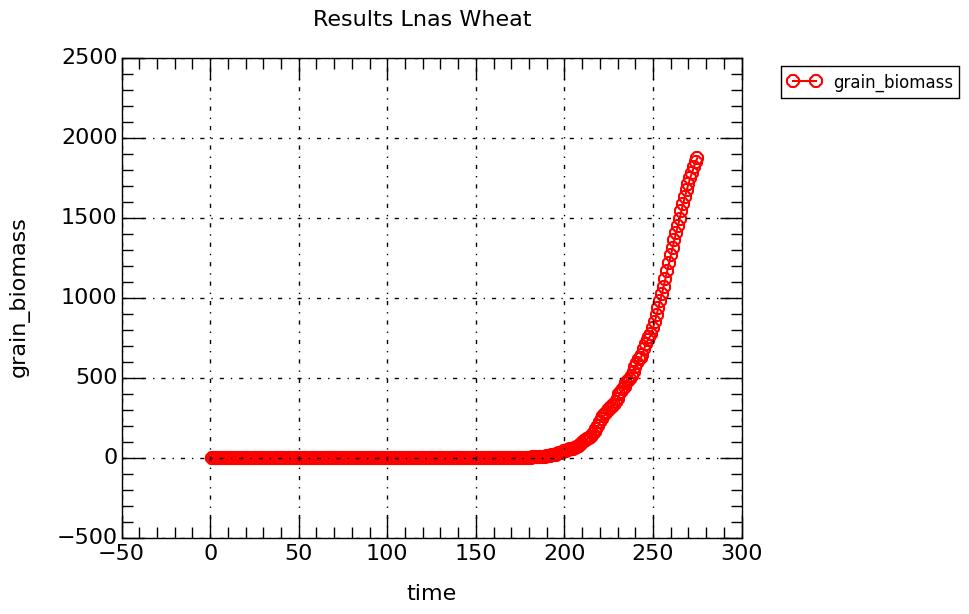
\includegraphics[scale = 0.67]{./img/grain.png}
 \caption{Biomasse de grain en fonction du temps.}
 \label{fig:resultatGrain}
\end{center}

\end{figure}

\begin{figure}[H]

\begin{center}
 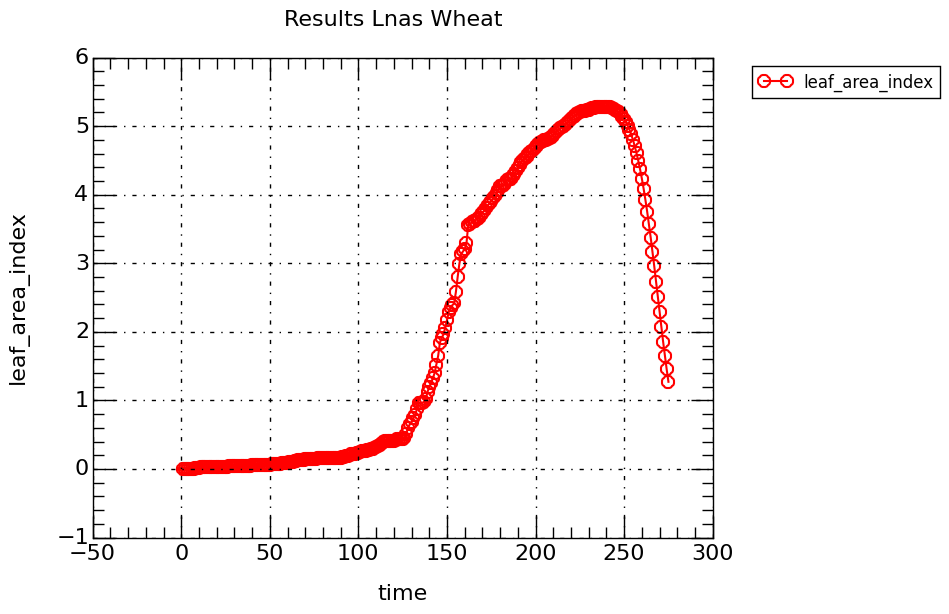
\includegraphics[scale = 0.67]{./img/LAI.png}
 \caption{Indice LAI en fonction du temps.}
 \label{fig:resultatLAI}
\end{center}

\end{figure}

\begin{figure}[H]

\begin{center}
 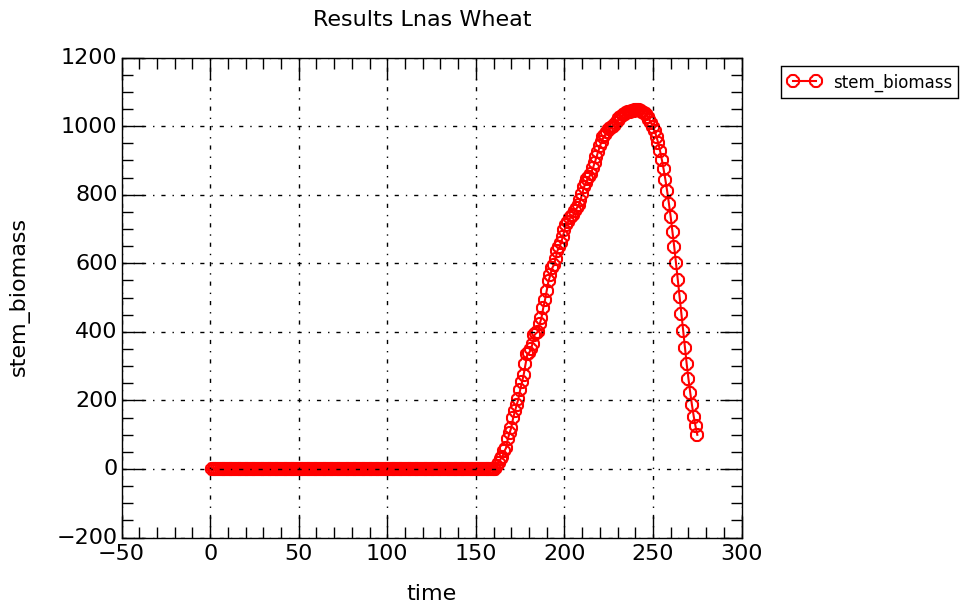
\includegraphics[scale = 0.67]{./img/stem.png}
 \caption{Biomasse de la tige en fonction du temps.}
 \label{fig:resultatStem}
\end{center}

\end{figure}

\begin{figure}[H]

\begin{center}
 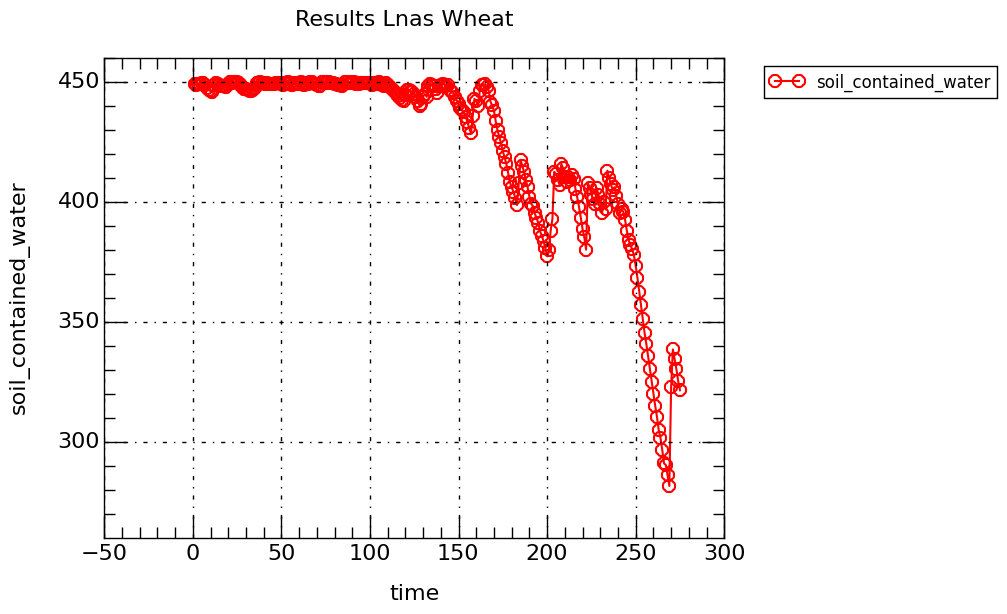
\includegraphics[scale = 0.67]{./img/water.png}
 \caption{Quantité d'eau dans la couche de sol considérée.}
 \label{fig:resultatWater}
\end{center}
\end{figure}

\begin{figure}[H]

\begin{center}
 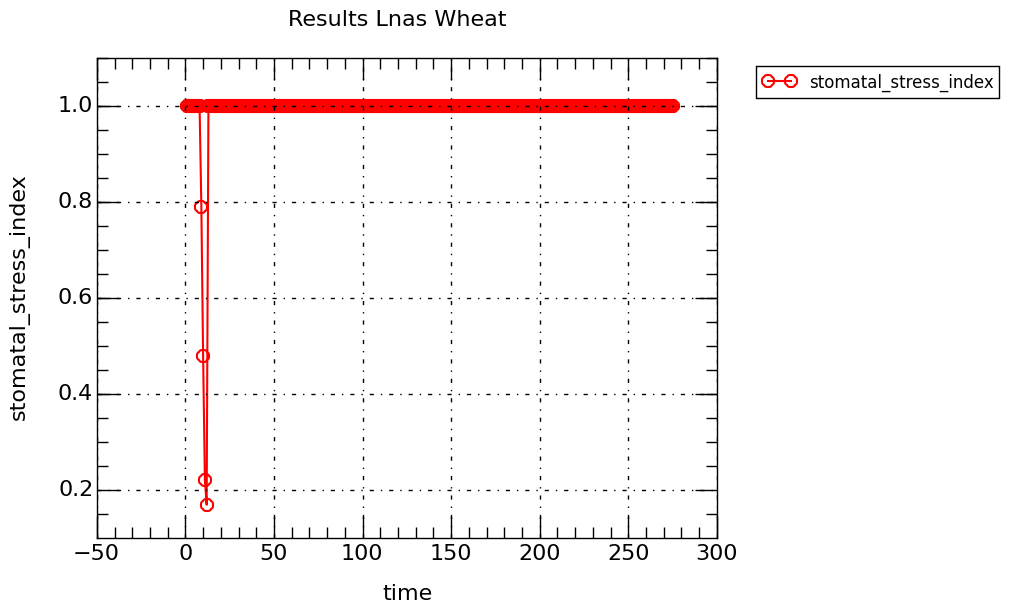
\includegraphics[scale = 0.67]{./img/waterStress.png}
 \caption{Indice de stress hydrique en fonction du temps.}
 \label{fig:resultatStressH}
\end{center}

\end{figure}

\begin{figure}[H]

\begin{center}
 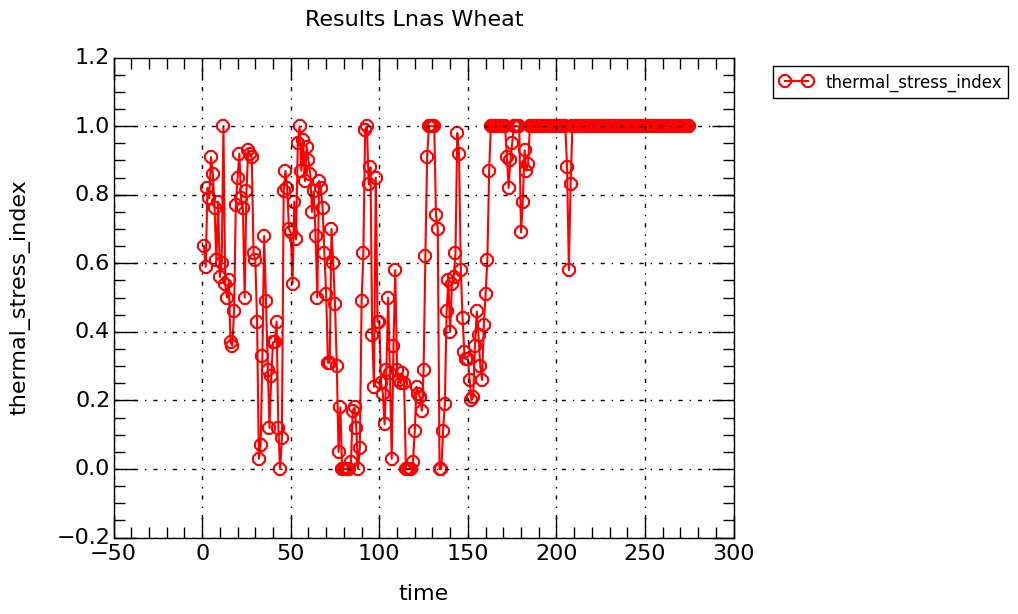
\includegraphics[scale = 0.67]{./img/thermicStress.png}
 \caption{Indice de stress thermique en fonction du temps.}
 \label{fig:resultatStressT}
\end{center}

\end{figure}

\subsubsection{Résultats et commentaires}

Pour ces différentes sorties, nous avons eu les résultats suivants :

\begin{itemize}
	\item \textbf{La masse du grain :} Nous avons un comportement qualitatif totalement cohérent : une croissance rapide et tardive de la quantité de grain. Cependant cette croissance dure trop longtemps et la quantité de biomasse du grain au moment de la récolte atteint des valeurs autour de 2000 au lieu de 1000. Les causes plausibles sont expliquées dans la partie méthodologie.
	
	\item \textbf{Le LAI :} Le résultat est à la fois très cohérent qualitativement et quantitativement. Le profil de la courbe correspond à celui qu'on trouve expérimentalement : croissance très rapide, croissance rapide, pic puis décroissance rapide. Et les valeurs maximum obtenues sont bien entre 5 et 6.
	
	\item \textbf{La masse des tiges :} Le comportement est cohérent et correspond à celui attendu : une croissance rapide à partir du temps de montaison puis une décroissance rapide avec la remobilisation et la sénescence. Il nous faudrait comparer avec des données expérimentales pour le quantitatif.
	
	\item \textbf{La quantité d'eau dans le sol :} Les réserves d'eau dans le sol sont larges au début et ne sont mises à mal par la plante que vers la fin alors qu'elle est déjà à maturité. Les paramètres environnementaux ne rendent pas la question de l'eau cruciale dans cette simulation : elle est abondante.
	
	\item \textbf{L'indice de stress hydrique :} La conclusion précédente est confirmée. La plante ne ressent à aucun moment de stress hydrique, à part un court épisode au départ dû à la longueur insuffisante de la racine mais rapidement corrigée. Pour mieux apprécier et évaluer la partie simulation de l'eau, on pourrait essayer le modèle avec des données environnementales qui présenteraient des périodes de sécheresse qui rendraient la question de l'eau plus cruciale.
	
	\item \textbf{L'indice de stress thermique :} Plus prévisible et direct que le stress hydrique, il est directement lié à la température. La simulation commence en hiver, le stress peut être ressenti avec des températures inférieures à 10, les épisodes de stress thermique sont donc surtout marqués en début de simulation, où ils peuvent ralentir la croissance de la plante, mais leur occurrence est normale en hiver et pas suffisamment sévère dans nos données pour empêcher la croissance normale de la plante.
\end{itemize}

Ainsi nous avons obtenu des résultats très satisfaisants qualitativement qui montrent que le modèle est fonctionnel et cohérent. Les comportements de sortie sont ceux attendus. La quantité de grain obtenue en sortie reste trop importante pour être réaliste et nous devons améliorer le modèle sur ce point. Les autres résultats quantitatifs sont satisfaisants.


\subsection{Perspectives}

Notre objectif premier, qui était d'implémenter le modèle LNAS appliqué au blé sur la plateforme Pygmalion-Julia, étant atteint, il s'agira après la soutenance de continuer le projet en affinant le modèle, en l'étudiant et en l'utilisant sur un jeu de données expérimentales pour comparer les simulations du modèle aux données réelles.

Ainsi, nous envisageons par exemple de décrire de manière plus précise le comportement de l'eau dans le sol. Ainsi, nous pourrions introduire dans le modèle la capillarité de l'eau, qui a tendance à la faire remonter des couches les plus humides aux couches les plus sèches, et décrire plus précisément le drainage de l'eau vers le bas dû tout simplement à la pesanteur. Il s'agira de comparer le comportement du modèle avec et sans ce raffinement, afin de constater ou non son utilité.

Pierre Carmier nous enjoint également à réaliser une analyse de sensibilité, pour déterminer l'influence de chaque paramètre sur le modèle. En effet, plus de 20 paramètres sont présents dans le modèle, et les déterminer tous nécessite de nombreux jeux de données. Si l'influence de certains paramètres s'avère assez faible, on pourra les remplacer par des constantes prises à leur valeur moyenne estimée pour simplifier l'étape de l'estimation des paramètres.

Nous aimerions également utiliser le modèle sur un jeu de données expérimentales. L'utilisation du modèle se décrit comme suit : on rentre un fichier de données expérimentales et on utilise une méthode d'estimation des paramètres (comme la méthode des moindres carrés généralisés par exemple, qui est déjà implémentée sur la plateforme). Cela nous permet d'obtenir une estimation des paramètres. 
Une fois les paramètres estimés, on utilise ceux-ci pour à nouveau réaliser des simulations avec 
le modèle. En effet, cette fois les paramètres sont fixés à leur valeur estimée et on ne rentre que les conditions initiales et extérieures du champ considéré.
Avec un autre jeu de donnée, on peut ainsi confronter les simulations obtenues avec les valeurs expérimentales. On vérifie ainsi la bonne adéquation du modèle, the goodness of fit. On peut ainsi obtenir le niveau d'incertitude de la prédiction fournie par le modèle.
Si cette étape s'avère concluante, on peut alors réaliser des prédictions sur à priori n'importe quel champ de blé. Ce sont les étapes logiques de modélisation. 




\newpage
%A mettre en annexe je pense
%\subsection{Estimation des paramètres}

Maintenant que le modèle est implémanté, il faut pouvoir estimer les paramètres qui interviennent dans le modèle, pour pouvoir utiliser le dit modèle.

Pour cela, nous utilisons une méthode déjà implémentée sur la plateforme ``lgs'', pour Generalized Least Squares (méthode des moindres carrés généralisée).

A partir des données expérimentales d'un champ de blé par exemple, cette méthode cherche les valeurs, les paramètres qui font converger les valeurs mesurées et les valeurs calculées par le modèle. 
La méthodes des moindres carrés généralisée est une méthode classique pour l'estimation de paramètres dans le cas de modèles déterministes, et c'est la cas ici puisque nous n'avons pas implémenté de bruit aléatoire dans notre modèle.

La méthode minimise la probabilité que les données expérimentales soient différentes de ce qui est prédit par le modèle. 
Mais, les calculs ne peuvent être conduits qu'en affectant une valeur arbitraire aux paramètres. On obtient ainsi une nouvelle valeur des paramètres, avec lesquelles on calcule de nouvelles valeurs des paramètres. Et ainsi de suite, jusqu'à que la valeur des paramètres converge.

L'avantage de cette méthode est son efficacité pour déterminer rapidement et avec une assez bonne précision les valeurs cherchées.
De plus, le fait que cette méthode soit déjà implémentée sur la plateforme est un autre avantage, puisque cela nous permet de l'utiliser sans avoir à l'implémenter. 


%\newpage
%\subsection{Markov}

Ces modèles sont des \emph{modèles de Markov} à temps discret. 
Soit $(t_{n}) n \in [0,N]$, la séquence finie des temps successifs correspondants
aux étapes de l’évolution. On note $X_{n}\in \reels^d$
l'ensemble des variables caractéristiques du système à $t_{n}$, $U_n \in \reels^u$
l'ensemble des variables exogènes (entrées, contrôle...) à $t_{n}$,
et $P\in R^p$ le vecteur de paramètres du modèle.
Comme pour la plupart des systèmes biologiques, $X_{n}$ peut ne pas être
complètement accessible à l'observation, et on note donc $Y_n \in \reels^{q_n}$
l'ensemble observé/mesuré des variables au temps $n$.
On note $Y=Y_n, n \in [0,N]$.
La fonction de densité initiale pour $X_0$ est $\mu_p$ 
et la densité de transition de Markov est $f_{n,P,U_n}$ :

\[
	X_0 \sim \mu_p \quad \text{ et } \quad
	 X_{n+1} \mid (X_n=x) \sim f_{n,P,U_n}(.\mid x)	\quad \forall n \in [0;N-1]
\]

L'observation $Y_n$ dépend de $X_n$ et la densité conditionnelle 
est donnée par $g_{n,P}$:
\[Y_n \mid (X_n = x) \sim g_{n,P} \]

Ce cadre stochastique permet d'aboutir et de décrire les modèles dynamiques discrets déterministes, en écrivant : 
\[
\left\{
    \begin{array}{ll}
        X_{n+1} &= F_n(X_n,U_n,P) \\
        Y_n &= G_n(X_n,P)
    \end{array}
\right.
\]

describes how an important category of plant growth models can be set in this framework. For example, for functional-structural models that describe biomass budget during plant growth (see for example LIGNUM [52] or GREENLAB [46]), the state variables correspond to daily biomass accumulation and to masses of plant organs according to their categories, the parameters are genotype specific, and the external variables Un correspond to environmental variables (radiation, temperature, soil water content ...).

Generally, not all the state variables can be observed experimentally (for example daily biomass pro- duction) and the experimentation being heavy (specifically when it comes to the masses of individual organs), observations are not done at all time steps. If we denote by O the set of all time step indexes corresponding to observation stages:
\[
  \mathcal{O} = \left\{i \in [1; N ] \text{ où } 
  t_i \text{ est un temps d'observation}\right\} 
\]
we then have qi > 0 if and only if i  O (where we recall that qi is the dimension of Yi). Note also that the non-zero qi have no reason to be identical (as illustrated for example in [45] for a model of maize growth, in which at some stages individual plants were measured at organ level, and at other stages only compartment data were available, corresponding to different Gi).

%1.1 Processus de Markov :
%
%Définition 1 : Le processus 〖〖(X〗_t)〗_(t≥0) est dit de Markov, si :
%	Pour tout t_1<t_2…< t_(n+1), pour tout x_1,…,x_(n+1)  :
%P(X_(t_(n+1) )=x_(n+1)∕X_(t_1 )=x_1,…,X_(t_n )=x_n )=P(X_(t_(n+1) )=x_(n+1)⁄X_(t_n ) =x_n)
%	Pour tout s et t, pour tout x,y∈E, P(X_(t+s)=y⁄X_s =x) ne dépend que de t.
%
%Remarque : L’axiome (1) (axiome de Markov) traduit que la probabilité de n’importe quel comportement futur, le présent étant connu, n’est pas modifié par toute connaissance supplémentaire du passé.

%\newpage
\section{Code et modèle}
\subsection{Description du modèle}

Le modèle LNAS blé est une version plus complexe du modèle LNAS betterave. Le modèle est constitué de deux compartiments principaux : le compartiment circulation de biomasse et le compartiment simulation de l'eau. Dans cette section nous ferons une explication des principes généraux et une description qualitative du modèle. Le lecteur intéressé trouvera tous les détails en annexe~\ref{ann:articlePierre} dans  la référence que nous avons nous-même utilisé pour implémenter le modèle.

\subsubsection{Circulation de biomasse}

\begin{figure}[H]

\begin{center}
 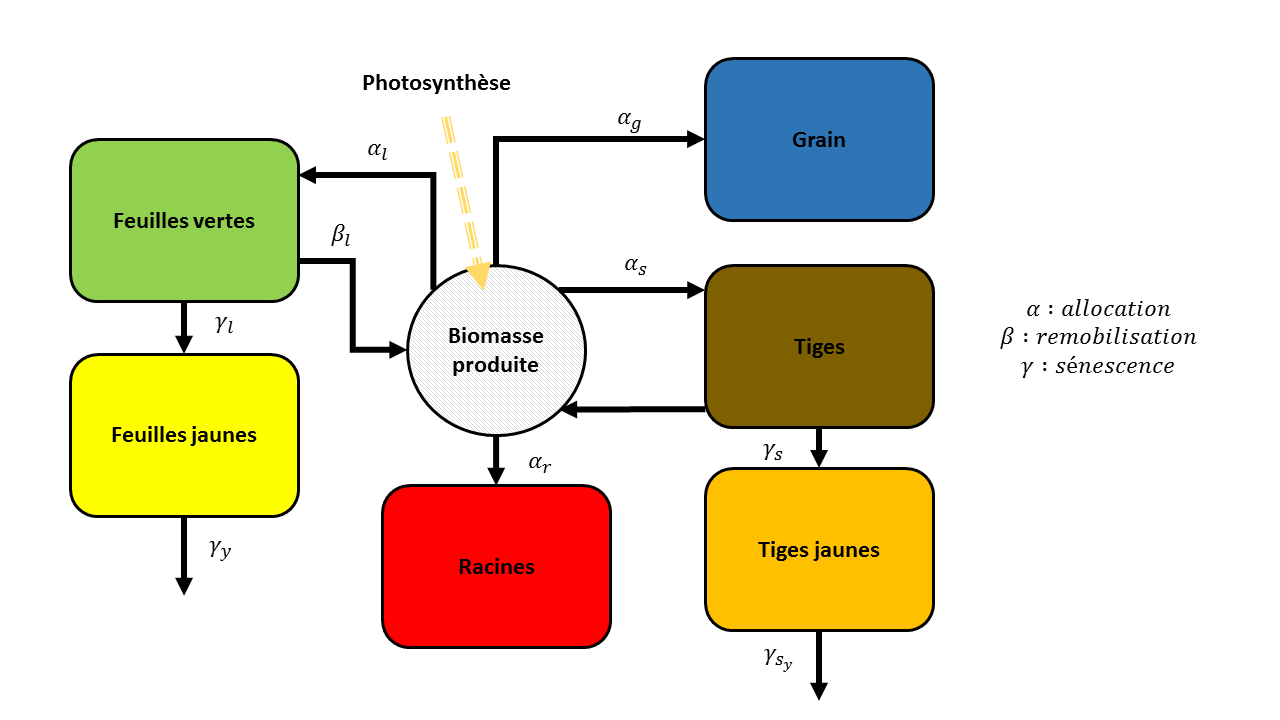
\includegraphics[scale = 0.42]{./img/modelSchema.png}
 \caption{Schéma de la circulation de biomasse.}
 \label{fig:schemaModel}
\end{center}

\end{figure}

Le modèle va à chaque itération calculer la quantité de biomasse produite, l'ajouter à un pool de biomasse. Ensuite il va calculer des coefficients d'allocation, de remobilisation et de sénescence qui vont déterminer la circulation de biomasse entre les différents compartiment, la loi de conservation voulant que toute la biomasse soit allouée au final. 
Les coefficients d'allocations déterminent la part de biomasse distribuée à chaque compartiment. Les coefficients de sénescence représentent un processus de vieillissement. Les coefficient de remobilisation représentent la part de biomasse des compartiment retournée au pool de biomasse pour être à nouveau alloué.

Les étapes sont les suivantes : 

\begin{itemize}

\item La biomasse est produite par photosynthèse et la quantité crée est calculée grâce à la loi de Beer-Lambert.  Un coefficient de stress hydrique et un coefficient de stress thermique peuvent réduire la production.

\item Des coefficients d'allocation sont ensuite calculés selon des lois log-normales, avec pour paramètres un temps caractéristique, à partir duquel l'allocation commence à être significative, une espérance et une variance. Typiquement, l'allocation aux racines et aux feuilles domine au départ, puis c'est celle aux tiges et vers la maturité de la plante c'est cella au grain.

\item Des coefficients de sénescence sont calculés selon des lois log-normales de la même façon. La sénescence des feuilles commence vers la fin de la croissance de la plante.

\item Enfin, des coefficients de remobilisation sont calculés toujours selon des lois log-normales. La remobilisation intervient de façon intense vers la fin pour les feuilles et les tiges en faveur du grain.

\end{itemize}

La valeur critique qui donne le rythme d'évolution de la plante n'est pas le temps réel mais le temps thermique qui correspond à l'accumulation de températures dépassant un certain seuil :
\[
\tau^{(n+1)} = \tau^{(n)} + \max[0, \underline{T^{(n)}} - T_c], 
\]
L'idée part d'un constat simple : la croissance de la plante est ralentie lorsque la température est basse.

\subsubsection{Simulation de l'eau}

\begin{figure}[H]

\begin{center}
 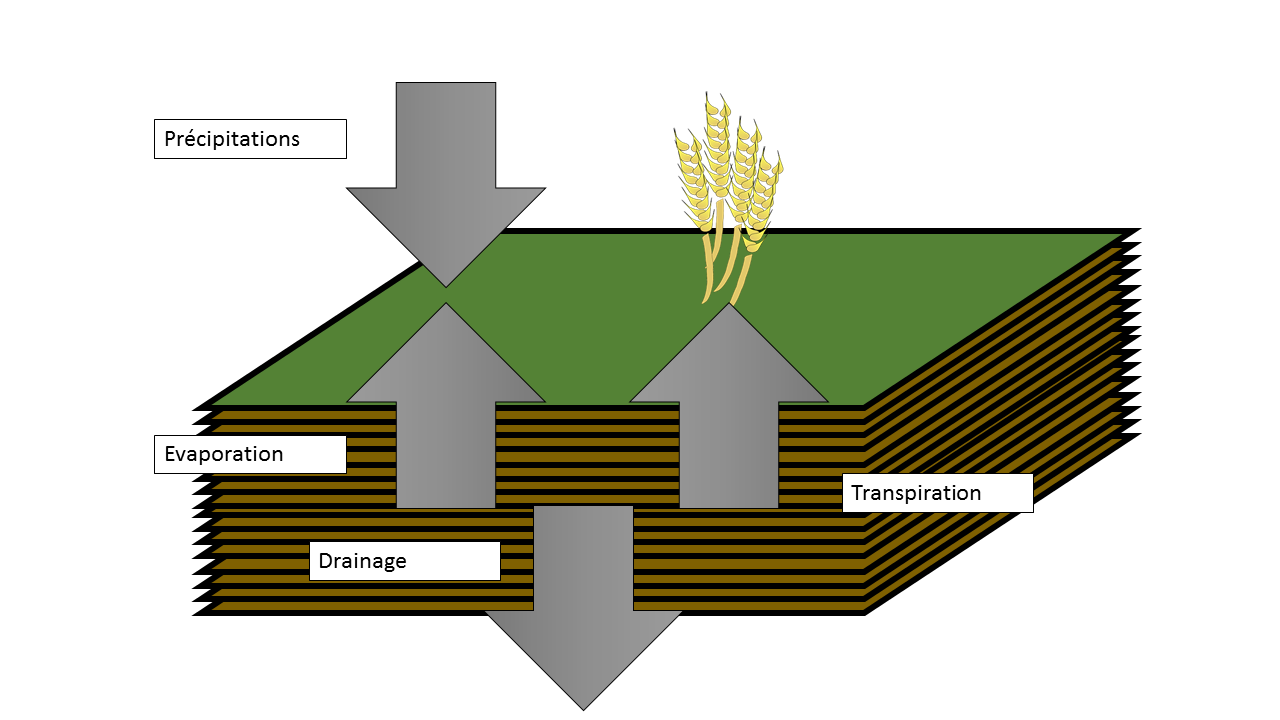
\includegraphics[scale = 0.42]{./img/waterSchema.png}
 \caption{Schéma de simulation de l'eau}
 \label{fig:waterModel}
\end{center}

\end{figure}

La simulation de l'eau est assez précisément décrite dans le modèle
et la figure~\ref{fig:waterModel} permet de comprendre intuitivement ce qu'il se passe. 

Elle repose sur l'équation d'équilibre de l'eau
\[ R^{(n+1)} = R^{(n)} + W^{(n)} - Es^{(n)} - Tp^{(n)} - d^{(n)}\]

Dans cette équation, $W^{(n)}$ représente les précipitations quotidiennes,
$Es^{(n)}$ est la quantité d'eau perdue par évaporation,
$Tp^{(n)}$ est la quantité d'eau transpirée par la plante 
et $d^{(n)}$ est une fonction de drainage qui évacue l'eau ne pouvant être absorbé si le sol est saturé. 

On calcule l'évaporation et la transpiration potentielles, qui sont la quantité d'eau pouvant être évaporée et transpirée en fonction de l'environnement (evapotranspiration du milieu, ensoleillement...). 
Puis l'évaporation et la transpiration ``max'' qui sont celles requises étant donnée la plante et l'environnement (profondeur des racines, ensoleillement...). 
On regarde donc la transpiration et l'évaporation qui aura effectivement lieu, qui sera le minimum entre le potentiel et ce qui est demandé.
Si la transpiration requise pour la plante n'est pas satisfaite, il y aura un stress hydrique. 

Une fois l'évaporation et la transpiration déterminée on rajoute au sol l'eau apportée par les précipitations puis on enlève l'eau évaporée puis transpirée. Les apports et pertes d'eau se font en FIFO (First In, First Out) ou ``piles'' : l'eau est d'abord rajoutée sur les couches supérieures jusqu'à saturation à l'humidité maximale (humidité au delà de laquelle le sol ne peut plus absorber d'eau) avant d'être rajoutée aux couches les plus basses, de même, on retire l'eau des couches supérieures d'abord jusqu'à atteindre l'humidité minimale (humidité en deçà laquelle on ne peut plus tirer d'eau), avant de retirer l'eau des couches les plus basses.
Tout excès éventuel d'eau après opérations est drainé.
\newpage
\subsection{Description du fonctionnement du code}
Dans un premier temps, nous avons construit un modèle informatique à partir
du modèle mathématique fourni~\cite{lnas_model_wheat}.

Il s'agissait d'abord d'affecter à chaque variable du modèle un représentant
dans notre programme, en rendant ces derniers assez explicites
afin d'être plus efficace pour l'implémentation des fonctions.
Les tableaux~\ref{table:state_var},~\ref{table:control_var} et~\ref{table:param_var}
contiennent respectivement les variables d'\emph{état}, temporaires, auxiliaires et principales, 
les variables \emph{environnementales} et les \emph{paramètres} de la tige, du sol et des racines.

La deuxième partie du travail consistait à définir les différentes fonctions (appelées ``modules'' selon les conventions Pygmalion)
qui mettent à jour les variables d'état et paramètres du 
temps $n$ au temps $n+1$.
L'implémentation de chacune d'entre elles est basée sur l'algorithme générique~\ref{lst:genfun}.
On retrouve à l'entrée les variables d'états \texttt{xn} et \texttt{xnplus1},
le temps \texttt{n}, les variables de contrôles \texttt{u}, les paramètres \texttt{p}.
On va ensuite mettre à jour une composante de \lstinline|xnplus1| par rapport à \texttt{xn} en fonction de \texttt{n}, \texttt{u} et \texttt{p} en suivant la description du modèle.

\begin{algorithm}[h]
  \caption{Algorithme générique qui sert de base pour l'implémentation
des fonctions. La fonction $f$ n'est pas définie mais sert de placeholder
pour représenter les opérations nécessaires à la mise à jour de \lstinline|xnplus1|.}
\label{lst:genfun}
  \begin{algorithmic}[1]
    \Procedure{Generic}{int $n$, State Vector $xn$, Control Vector $u$, Parameters Vector $p$, State Vector $xnplus1$}
    \State \textbf{begin}
      \State $xnplus1.composante \gets f(p.composante, u.composante, xn.composante)$
    \State \textbf{end}
    \State \textbf{return} None
    \EndProcedure
  \end{algorithmic}
\end{algorithm}

\lstset{        literate=
                       {==}{$={}$}{1}}

À titre d'exemple, on présente la fonction \lstinline|get_pot_evaporation| qui met
à jour l'évaporation requise en fonction des conditions environnementales
selon l'équation~\ref{eq:req_evap}.
\begin{equation}
  \text{Espot}^{(n)} = K_s \text{ ET0 } e^{-\lambda \text{ LAI}^{(n)}}
  \label{eq:req_evap}
\end{equation}
On obtient en \textsc{Julia} l'implémentation suivante
\begin{lstlisting}
function get_pot_evaporation!(n, xn, u, p, xnplus1)
  xnplus1.soil_req_evaporation = 
    p.k_s * u.ET0[n] * exp( -p.lambda * xn.leaf_area_index) 
end
\end{lstlisting}

Il reste finalement deux fonctions particulières qui ne suivent
pas l'algorithme~\ref{lst:genfun}.
% Elles se nomment \lstinline|initialize|, \lstinline|transition|
% et servent respectivement à initialiser \lstinline|xn| et
% à exécuter toutes les fonctions pour passer au temps suivant.

\begin{enumerate}
  \item \lstinline|initialize| qui va initialer les composantes de \lstinline|xn|,
  \item \lstinline|transition| qui permet de passer au temps suivant et d'exécuter toutes les fonctions.
\end{enumerate}




\begin{table}[h]
  \centering
  \begin{tabular}{c|c}
    \textbf{Modèle mathématique} & \textbf{Implémentation} \\
    $Q_r$ & root\_biomass \\
    $Q_s$ & stem\_biomass \\
    $Q_l$ & green\_leaf\_biomass \\
    $Q_g$ & grain\_biomass \\
    $Q_y$ & yellow\_leaf\_biomass \\
    $\theta$ & soil\_humidity \\
    $\tau$ & thermal\_time \\
    $R$ & soil\_contained\_water \\
    $E_s$ & soil\_water\_evaporated \\
    $T_p$ & water\_transpired \\
    $z_r$ & root\_horizon \\
    SSI & stomatal\_stress\_index \\
    TSI & thermal\_stress\_index \\
    TSI$_{\uparrow}$ & thermal\_stress\_index \\
    TSI$_{\downarrow}$ & soil\_thermal\_stress\_index \\
    % Auxiliary
    $q$ & produced\_biomass \\
    LAI & leaf\_area\_index \\
    E\textsubscript{spot} & soil\_req\_evaporation \\
    T\textsubscript{ppot} & req\_transpiration \\
    E\textsubscript{smax} & soil\_max\_evaporation \\
    T\textsubscript{pmax} & max\_transpiration \\
    T$_{\downarrow}$ & soil\_temperature \\
    % Temporary
    $\alpha_g$ & alpha\_g \\
    $\alpha_s$ & alpha\_s \\
    $\alpha_r$ & alpha\_r \\
    $\alpha_l$ & alpha\_l \\
    $\beta_s$ & beta\_s \\
    $\beta_l$ & beta\_l \\
    $\gamma_l$ & gamma\_l \\
    $\gamma_y$ & gamma\_y \\
  \end{tabular}
  \caption{Variables d'\emph{état} du modèle mathématique et leurs noms
  dans l'implémentation.}
  \label{table:state_var}
\end{table}

\begin{table}
  \centering
  \begin{tabular}{c|c}
    \textbf{Modèle mathématique} & \textbf{Implémentation} \\
    $T$ & vec\_ext\_temperature \\
    PAR & vec\_par \\
    $W$ & vec\_water\_input \\
    ET0 & vec\_et0 \\
  \end{tabular}
  \caption{Variables de \emph{contrôle} du modèle mathématique et leurs noms
  dans l'implémentation.}
  \label{table:control_var}
\end{table}

\begin{table}
  \centering
  \begin{tabular}{c|c}
    \textbf{Modèle mathématique} & \textbf{Implémentation} \\
    $t_c$ & t\_c \\
    $t_{opt}$ & t\_opt \\
    $\mu_g$ & mu\_g \\
    $\sigma_g$ & sigma\_g \\
    $\eta_s$ & eta\_s \\
    $\eta_l$ & eta\_l \\
    $\tau_l$ & tau\_l \\
    $\mu_l$ & mu\_l \\
    $\sigma_l$ & sigma\_l \\
    $\tau_y$ & tau\_y \\
    $\mu_y$ & mu\_y \\
    $\sigma_y$ & sigma\_y \\
    RUE & rue \\
    $\lambda$ & lambda \\
    $\rho_l$ & rho\_l \\
    $K_c$ & k\_c \\
    $K_s$ & k\_s \\
    $\theta_{max}$ & theta\_max \\
    $\theta_{min}$ & theta\_min \\
    $z_s$ & z\_s \\
    $z_m$ & z\_m \\
    $\rho_r$ & rho\_r \\
    $t_{\downarrow c}$ & t\_soil\_c \\
    $t_{\downarrow opt}$ & t\_soil\_opt \\
  \end{tabular}
  \caption{Paramètres du modèle mathématique et leurs noms
  dans l'implémentation.}
  \label{table:parameters_var}
\end{table}
  







\newpage
\section{Conclusion}

\newpage
\section*{Remerciements}
\addcontentsline{toc}{section}{Remerciements}

Nous tenons tout d'abord à remercier notre client Pierre Carmier,
pour sa pédagogie et son temps précieux accordé. 
Nous remercions également Mme Le Chevalier et Mme Lopes, qui encadrent
le projet de façon motivante et efficace.
Leurs remarques et retours sur nos présentations 
ainsi que sur l'avancement de notre projet
nous ont été très utiles pour prendre le recul
nécessaire à la rédaction de ce rapport.
Enfin, merci à nos responsables d'ateliers Mme Lévy et M. Bertrand, qui nous ont permis de mieux appréhender l'aspect humain du projet, que ce soit pour présenter à l'oral ou communiquer au sein du groupe.
\newpage
 
 
\addcontentsline{toc}{section}{Bibliographie}
\nocite{*}
\printbibliography
\newpage

\part*{Annexes}
\appendix
\section{Physiologie des plantes}
\label{ann:physiologie}

\subsection{Fonctionnement et développement de la plante}

\subsubsection{Généralités}

Tout d'abord, présentons succintement comment se développe et fonctionne une plante. 
La science qui décrit l'ensemble des mécanismes qui participent à l'édification d'un organsime vivant est appelée morphogénèse

Chez les plantes, la morphogénèse commence avec la germination de la graine et s'arrète à la mort de la plante.~\cite[p.~22]{these_modelisation}.
Celle-ci diffère d'une plante à l'autre, et dépend également de l'environnement de la plante.

Ce sont les méristèmes\footnote{Le méristème est un tissu formé de cellules indiffériencées (embryonnaires) qui se divisent activement et permettent la croissance.} qui permettent à la plante de se développer, en allongeant des organes déjà existants ou en créant de nouveaux organes.
Lors de la germination de la graine, au stade embryonnaire, des méristèmes permettent déjà le développement de la plante (méristèmes racinaires, caulinaires).
On distingue les méristèmes végétatifs, à l’origine des organes végétatifs (tige, feuilles, racines) et les méristèmes reproducteurs, à l’origine des fleurs.
On distingue également les méristèmes primaires, qui permettent à la plante de croître en longueur (tiges et racines) et les méristèmes secondaires, qui permettent la croissance en épaisseur de la plante.
La création de nouveaux organes est réalisée par alignement de nouvelles briques élémentaires (formée par les méristèmes), constituées :
\begin{itemize}
	\item d'un noeud, auquel sont liés les feuilles
	\item d'un entrenoeud 
	\item d'un bourgeon situé à la base du noeud, à l'aisselle des feuilles
\end{itemize} 

Ces briques élémentaires sont appelées phytomères. Cette caractéristique permet de simplifier la modélisation de la croissance d'une plante.



\subsubsection{Photosynthèse}
\label{subsubsec:photosynthese}
Sans doute que la particularité la plus intéressante des plantes, et qui justifie le mieux leur étude est leur capacité à synthétiser de la matière organique (des glucides...) à partir de \ce{CO2}, d'eau et d'énergie solaire. C'est la célèbre photosynthèse qui permet ainsi à la plante de 
transformer de la matière \emph{minérale} en matière \emph{organique},
selon l'équation
\begin{equation}
	\ce{6CO2 + 6H2O + \text{énergie solaire} -> C6H12O6 + 6O2 }.
  \label{eq:photosynthese}
\end{equation}

Tous les éléments de la plante participent à ce processus de photosynthèse :
\begin{itemize}
	\item les racines puisent dans le sol l'eau et les sels minéraux nécessaires		
	\item les feuilles captent l'énergie solaire et le dioxyde de carbone 
  (grâce aux cellules chlorophiliennes 
  et aux stomates\footnote{Orifice de petite taille situé sur les feuilles 
  qui permet les échanges gazeux entre l'air et la plante.})
\end{itemize}

\begin{figure}[h]
	\begin{center}
  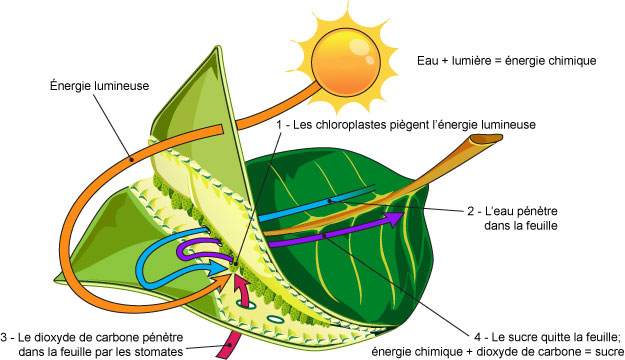
\includegraphics[scale=0.51]{./img/photosynthese.jpg}
  \caption{Schéma de la photosynthèse illustrant les différents 
  mécanismes qui permettent à celle-ci d'avoir lieu.}
  \label{fig:photosynthèse}
	\end{center}
\end{figure}

Les sucres ainsi formés apportent l'énergie nécessaire au fonctionnement de la plante et assurent son développement en permettant la synthèse de cellulose qui est l'élément consitutif principal des plantes.
On identifie ainsi les éléments qui agissent sur la croissance de la plante : 
\begin{itemize}
	\item la lumière
	\item l'eau
	\item le dioxyde de carbone
	\item la température : car la température agit sur l'ouverture des stomates et donc sur le flux des échanges gazeux
	\item l'azote, qui permet à la plante de construire les acides aminés nécessaires à l'élaboration des protéines
	\item d'autres minéraux, comme le potassium qui favorise les transferts au sein de la plante
\end{itemize}

Tous les organes de la plante s'unissent donc pour aboutir à la production de biomasse. Cette biomasse est ensuite distribuée aux organes pour permettre leur développement.

Parce que ce mécanisme permet de synthétiser de la matière minérale en matière organique et de capter du \ce{CO2}, gaz à effet de serre notoire, il est crucial de comprendre ce mécanisme de photosynthèse. C'est pourquoi il est, au même titre que la croissance des plantes l'objet de nombreuses recherches (avec comme application : créer de l'électricité propre en dissociant \ce{H2O} en Oxygène et en Hydrogène, capter du \ce{CO2}...

	

 \newpage
\section{Histoire de la modélisation de la croissance des plantes}
\label{ann:histoire}

Nous présentons dans cette partie tout d'abord l'origine
de la botanique et de l'agronomie. Les premièrs modèles
de croissance des plantes seront ensuite décrits,
puis on expliquera les avancées potentielles apparues avec
l'avènement de l'informatique.
Finalement, un modèle particulièrement intéressant,
le modèle GreenLab, sera présenté.

Cette section reprend la démarche suivie dans 
l'article \emph{Une histoire de la modélisation des plantes}, \textsc{Cournède} et al., 2009~\cite{histoire_mod_plantes}.

\subsection{Débuts de la botanique et de l'agronomie}
L’étude des plantes a très tôt été un domaine privilégié du savoir humain.
En effet, les plantes sont un élément majeur des écosystèmes dans lesquels l’homme évolue. Elles sont source de nourriture, de remèdes, de médicaments,
de matériaux, d’esthétique. 
Enfin, elles sont un objet scientifique d’intérêt qui a très tôt aiguisé le sens de l’observation, l’esprit d’analyse, de synthèse, de déduction des hommes. 
La connaissance des plantes s’est accrue lors de l’histoire des hommes, qui ont développé la cueillette, l’agriculture, l’usage des plantes
médicinales. 
La connaissance et l’inventaire des variétés de plante ont ainsi été des
enjeux majeurs car ils permettaient la connaissance de nouveaux remèdes
et étaient sources de nourritures et matériaux. 
L’homme a ainsi cherché à regrouper, croiser, faire croître 
et conserver les espèces qui lui étaient utiles.

La botanique, issue de l’étude de l’anatomie des plantes,
est une science très ancienne.
En témoignent les traités de classification de plantes, comme ceux
d’Aristote (vers -300), ou encore l’inventaire et la description de
centaines de plantes médicinales par Dioscoride (1er siècle),
ainsi que les traités chinois qui inventorient les espèces utiles à
l’agriculture et à la médecine traditionnelle avec de premiers efforts
de classification. 
Efforts de classification qui se poursuivront vraiment en Europe à partir du
XVIIème siècle avec les premières distinctions par famille, par genre,
par espèce, par structure de graine (\emph{Les éléments de Botanique} par
Joseph Pitton de Tournefort en $1656-1708$, \emph{Systema naturae} en 1735
et \emph{Philosophia botanica} en 1751 par Linné et les travaux de la
famille de Jussieu pendant le XVIIIème siècle).
Ces classifications ne sont pas objectives, 
elles sont le fruit d’un raisonnement \emph{empirique}.

En parallèle, l’agronomie se développe au XVIIème siècle en Europe
et s’intéresse au processus de croissance et développement des plantes.
Des travaux d’abord très pratiques sont réalisés sur des méthodes agricoles 
(labour, ensemencement, taille, greffes…), notamment ceux de
Jean-Baptiste de la Quintinie et d'Olivier de Serres.

Au XIXème, les processus biologiques commencent à être étudiés de façon plus
précise, en particulier la provenance du carbone, de l’azote,
de l’oxygène et de l’eau dans la plante.
On s'intéresse également aux problématiques de nutrition et
au rôle de organes, comme en témoignent les ouvrages
\emph{Recherces chimiques sur la végétation} de Théodore de Saussure en 1804.
Quelques années plus tard, on découvre la respiration, la photosynthèse
(voir équation~\ref{eq:photosynthese} à la 
page~\pageref{subsubsec:photosynthese}).

La physiologie, science qui étudie le fonctionnement des plantes,
se sépare alors de la botanique qui se contente de les classifier.

\subsection{Les premiers modèles}

La modélisation mathématique précise (qui va au-delà de la simple
description qualitative et fournit une description quantitative
avec des capacités prédictives) n’arrive pas tout de suite en biologie. 
Le développement de la biologie n’a pas suivi le même schéma que celui de
nombreuses autres sciences comme la physique, où l’observation a permis de
tirer des concepts quantitatifs au niveau macroscopique
(loi de Mariotte par exemple) avant de les expliquer par des lois qui s’appliquent au niveau microscopique (Boltzmann). De même pour la mécanique, l’optique, l’électricité avec des applications qui n’ont pas eu à attendre la compréhension au niveau atomique. La biologie végétale par contre a paradoxalement été mieux comprise au niveau cellulaire et microscopique sans que des lois précises macroscopiques en soient tirées.

Trois types de modèles vont se développer et vont changer cela : les modèles de l’architecture botanique, les modèles de production en agronomie et les modèles géométriques en informatique. Ainsi la convergence de ces trois modèles initialement séparés va permettre récemment les débuts de la modélisation précise de la croissance des plantes à la fin du XXème siècle.  

L’architecture botanique va considérer la structure des plantes non plus comme une description statique issue de la classification traditionnelle mais comme le résultat de l’organogénèse des méristèmes, la cinétique de mise en place des axes feuillés, en se basant sur une combinatoire des modes de croissance, de ramification et de floraison. (Francis Hallé et Roelof Oldeman).

En parallèle, l’agronomie s’est attaquée à la prédiction de la production surfacique de biomasse. Les modèles hollandais comme celui de De Witt (1970) en sont les précureurs. On ne considère plus la plante en elle-même mais la surface foliaire au mètre carré LAI\footnote{LAI : Leaf Area Index.
Cela correspond au ratio entre la surface totale supérieure des feuilles
vertes et la surface de sol sur laquelle se développe la culture.} 
et la production végétale par mètre carré.
Les organes ne sont plus considérés individuellement mais par compartiments. A chaque compartiment est allouée une certaine quantité de la biomasse créée en fonction de sa force de 
puits.
La force de puits d'un organe est proportionelle à la quantité de biomasse qui sera allouée à cet organe.\cite[~p.229--231]{hopkins2003physiologie}

Les agronomes ont ainsi montré que la production de biomasse est proportionnelle au LAI, ainsi qu'à l’énergie utile de la lumière incidente : PAR \footnote{PAR : Photosynthetically Active Radiation.}, à la lumière interceptée : I et à un facteur d’efficience énergétique : LUE\footnote{LUE : Light Use Efficiency.}. On se reporte à la loi de Beer-Lambert pour trouver la quantité de lumière interceptée, qu'on note I : 

\[ I = 1-e^{-k\cdot\mathrm{LAI}} \]

Ce qui permet ensuite de trouver la production de biomasse $Q$
en déterminant le LUE et en mesurant la PAR.
\[ 
  Q = \mathrm{LUE}\times\mathrm{PAR}\times I 
\]

Dernier concept empirique développé, celui de temps thermique
\footnote{Le temps thermique correspond à l'accumulation de températures dépassant un certain seuil :
\[
\tau^{(n+1)} = \tau^{(n)} + \max[0, \underline{T^{(n)}} - T_c], 
\]

où $\underline{T^{(n)}}$ est l'écart de température constaté et 
$T_c$ est le seuil de variation de température qu'on impose.
}.
En effet, si on modélise la croissance de la plante  en fonction du temps, cette croissance est très irrégulière et se fait par à coup. Mais si l’on considère le temps thermique on peut trouver une relation quasi-linéaire.


 \newpage
\section{Développement et évaluation des modèles de croissance des plantes}
\label{ann:caracteristique}

\subsection{Généralités}

Les modèles mathématiques de modélisation de la croissance des plantes sont généralement caractérisés par un grand nombre de processus en interaction,  un grand nombre de paramètres et une acquisition coûteuse des données expérimentales. 
Nous présentons des éléments de bonnes pratiques de modélisation, afin de donner un aperçu global des différentes étapes de modélisation dans le cadre de la croissance des plantes.
Le modèle LNAS (celui sur lequel on travaillera en premier dans le cadre du projet enjeu) est présenté comme illustration de ces méthodes, ici appliqué à la betterave, et montre comment il peut être paramétré, évalué et appliqué à la prédiction des rendements, et ce à travers des données expérimentales réelles. Ce modèle a d’intéressante capacité de prédiction lorsqu’il est couplé a de bonnes méthodes d’acquisition de données.

\subsubsection{Caractéristiques propres aux modèles de croissance de plantes}

\begin{itemize}

\item \textbf{Une complexité importante} au niveau des processus et des paramètres
\item \textbf{Une paramétrisation difficile} à cause de cette complexité ainsi que du coût important des données.
\item \textbf{Un besoin croissant} en techniques sophistiquées en informatiques, mathématiques et statistiques.
\item \textbf{Une importante diversité} de modèles existants sans benchmarking entre les différentes approches (lacune de méta-études statistiques)

\end{itemize}

Les solutions mathématiques et statistiques classiques et généralistes ne sont pas immédiatement adaptées à la modélisation des plantes et nécessitent un travail d’adaptation important pour prendre en compte ses spécificités.

D’un autre côté les logiciels de modélisations spécialisés, bien que performant, ne prennent pas assez en compte l’aspect paramétrisation et évaluation statistiques.

Les logiciels développés récemment dans ce domaine offrent des solutions intéressantes mais elles sont peu compatibles entre elles et limitent donc la comparaison, le benchmarking des modèles.

L’objectif est donc à la fois bien de situer les bonnes pratiques de modélisation, et de proposer une implémentation pratique, notamment à travers la plateforme Pygmalion en C++ qui fournit un template générique de modèle, des structures de données, des méthodes, des classes et framework appropriés, ainsi qu’une méthodologie statistique.

\subsubsection{Bonnes pratiques en modélisation}

\begin{itemize}

\item \textbf{Analyse du modèle :} Etude des comportements généraux du modèle, au niveau théorique et numérique par des simulations. Pour déterminer les données nécessaires à la paramétrisation, et faire une analyse de sensibilité pour repérer les paramètres importants.
\item \textbf{Identification du modèle :} Confronter les modèles à des données expérimentales. Identification de la structure : pour identifier dans la famille du modèle la plus intéressante. Identification des paramètres : pour identifier la valeur des paramètres pour la structure choisie.
\item \textbf{Evaluation du modèle :} Vérifier qualitativement (comportement générale et aptitude de simulation) et quantitativement (comparaison aux données réelles) si le modèle atteint ses objectifs, c’est-à-dire vérifier la correspondance aux donnée actuelles (goodness of fit), tester ses capacités prédictives et évaluer son niveau d’incertitude.

\end{itemize}

\textbf{Ces étapes ne sont pas linéaires :} des allers retours sont nécessaires pour ajuster finement le modèle.

%Ensuite ces étapes sont appliquées au modèles LNAS avec des jeux de données expérimentales, avec succès, en notant des capacités prédictives intéressantes dans un cadre données expérimentales très différent de celui utilisé lors de la calibration du modèle.
%Cette première étape développée par le laboratoire MAS de l’ECP, montre l’intérêt de la démarche, et invite à l’appliquer avec d’autres modèles, d’autres plantes et sur d’autre jeux de données tout en continuant d’améliorer la plateforme, tout en simplifiant son utilisation.

 \subsection{Modèle LNAS appliqué à la betterave}
 
-Le modèle LNAS (Long Normal Allocation and Senescence) appliqué à la betterave. C’est un modèle innovant et suffisamment simple pour illustrer tous les enjeux de la thèse. Il est plutôt robuste étant donné sa simplicité, et le faible nombre de données et paramètre requis le rend pratique à l’utilisation. Il traite la production de biomasse au niveau compartemental et peut être considéré comme une simplification du modèle Digiplante qui décrit les même processus au niveau des organes.
+Le modèle LNAS (Long Normal Allocation and Senescence) appliqué à la betterave. C’est un modèle innovant et suffisamment simple pour illustrer tous les enjeux de la thèse. Il est plutôt robuste étant donné sa simplicité, et le faible nombre de données et paramètre requis le rend pratique à l’utilisation. Il traite la production de biomasse au niveau compartemental et peut être considéré comme une simplification du modèle Greenlab qui décrit les même processus au niveau des organes.
 C’est un modèle Markovien en temps discret.
 
 \begin{figure}[h]
 	\begin{center}
 	
 	
   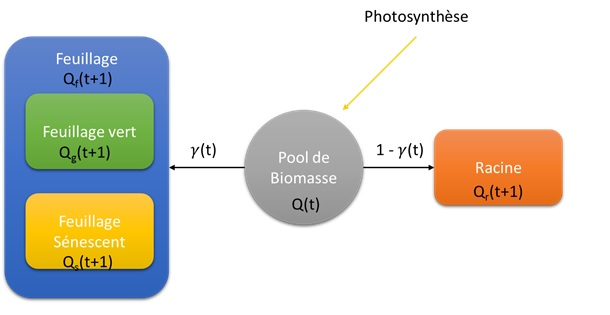
\includegraphics[scale=1.0]{./img/sBeetRoot.jpg}
   \caption{Schéma du modèle LNAS appliqué à la betterave}
   \label{fig:sBeetRoot}
   
   \end{center}
 \end{figure}
 
+Production de Biomasse :
 \[ \mathrm{Q}(t) = \big(\mu\cdot\mathrm{PAR}(t)(1-e^{-\lambda\mathrm{Q_g}(t)}\big)\cdot(1+\mathrm{\eta_Q}(t)) \]
 
+Allocation au feuillage :
 \[ \mathrm{Q_f}(t+1) = \mathrm{Q_f}(t) + \mathrm{\gamma}(t)\cdot\mathrm{Q}(t) \]
 
+Allocation à la racine :
 \[ \mathrm{Q_r}(t+1) = \mathrm{Q_r}(t) + (1 -\mathrm{\gamma}(t))\cdot\mathrm{Q}(t) \]
 
+Fonction d'allocation :
 \[ \mathrm{\gamma}(t) = (\gamma_0 + (\gamma_f - \gamma_0)\cdot\mathrm{G_a}(\mathrm{\tau}(t)))\cdot(1+\mathrm{\eta_{\gamma}}(t)) \]
 
+Fonction de sénescence :
 \[ \mathrm{Q_s}(t) = \mathrm{G_s}(\mathrm{\tau}(t)- \tau_{sen})\mathrm{Q_f}(t) \]
 
+Part de la biomasse produite qui arrive aux feuilles vertes :
 \[\mathrm{Q_g}(t) = \mathrm{Q_f}(t) - \mathrm{Q_s}(t) \]
 
 \begin{itemize}
 
 \item $\mathrm{Q}(t)$ : Production de biomasse au jour t par unité de surface.
 \item $\mu$ : Efficacité énergétique
 \item $1-e^{-\lambda\mathrm{Q_g}(t)}$ : Fraction des radiations interceptées
 \item $\mathrm{PAR}(t)$ : quantité de radiations photosynthétiquement actives par unité de surface.
 \item $\lambda$ : paramètre
 \item $\mathrm{Q_g}(t)$ : masse total des feuilles vertes au jour t
 \item $\mathrm{Q_f}(t)$ : masse total du feuillage au jour t
 \item $\mathrm{Q_s}(t)$ : masse total du feuillage sénescent au jour t 
 \item $\mathrm{\gamma_0}, \mathrm{\gamma_f}$ : paramètres
 \item $\mathrm{\eta}(t)$ : variables aléatoires normales 
 \item $\mathrm{G}(t)$ : variables aléatoires lognormales
 \item $\mathrm{\tau}(t)$ : temps thermique au jour t (température cumulée depuis l'émergence de la plante)
 \item $\tau_{sen}$ : temps thermique où la sénescence commence.
 \item Les paramètres des variables aléatoires font parti des paramètres du modèle.
 
 \end{itemize}
 \newpage
\section{Quelques modèles de la croissance des plantes}
\label{ann:modele}

\subsection{Informatique et modèles géométriques}

L’arrivée des ordinateurs a révolutionné les méthodes de simulation ainsi que
de modélisation des systèmes et l’étude des plantes en a bien sûr profité.
Les ordinateurs ont fait leur apparition presque en même temps que les
modèles agronomes et botaniques. Ainsi, très vite, ils ont été vus comme un
moyen de simuler la structure géométrique complexe des plantes avec le
développement d’arbres combinatoires, binaires et fractals. 
Mais ces structures purement géométriques et trop rigides ne simulent pas
encore bien le développement complexe des plantes.
Les travaux d’Aristide Lindenmayer aboutissent à une grammaire au formalisme
puissant, grammaire générative basée sur le principe de
réécriture~\cite{LSystem}.

\noindent{
\fbox{
  \parbox{\textwidth}{\paragraph{Qu'est-ce qu'un L-Système?}
Un L-Système est noté :
\[ \{ V,S,\omega ,P \}  \]
Une grammaire formelle qui comprend :
\begin{itemize}
\item Un ensemble alphabet \textbf{V}: Ensemble de variable du L-Système
\item Un ensemble de constantes \textbf{S} : Ensemble de constantes servant notamment lors du dessin géométrique.
\item Un axiome de départ $\mathbf{\omega}$ : État initial.
\item Un ensemble de règles \textbf{P} : Règles de production.
\end{itemize}
Un exemple simple : Algues de Lindenmayer
\[ 
  \left\lbrace
		\begin{array}{cl}
		  V &= \{ A, B\} \\
		  S &= \{ \} \\
		  \omega &= A \\
		  P &= ( A\rightarrow AB)\wedge (B\rightarrow A) \\	
     \end{array}
   \right. 
\]
Avec le résultat sur 6 générations :

\begin{itemize}
  \item[$\bullet$] $n=0$, A
  \item[$\bullet$] $n=1$, AB
  \item[$\bullet$] $n=2$, AB A
  \item[$\bullet$] $n=3$, AB A AB
  \item[$\bullet$] $n=4$, AB A AB AB A
  \item[$\bullet$] $n=5$, AB A AB AB A AB A AB
  \item[$\bullet$] $n=6$, AB A AB AB A AB A AB AB A AB AB A
\end{itemize}

Une suite de symboles générée par L-Système peut être prise en entrée par un
programme informatique qui s’en servira pour générer une structure
géométrique, le plus simple étant d’utiliser un turtle en 2D voire en 3D,
ou encore dans un langage orienté objet avec des pointeurs on peut générer
une chaine cellulaire qui évolue. Les symboles dans $V$ sont les parties des plantes dessinées et les symboles dans $S$ donnent des informations sur la façon dont elles sont dessinées, leur orientation par exemple.
}   
}

Ces modèles de L-système conviennent bien à la simulation des structures des
plantes, elles marchent d’autant mieux combinées à la notion de temps
thermique qui ordonne la dynamique de croissance et permettent d’aboutir 
in fine à une architecture fidèle. On constante cependant
qu'elles n’intègrent pas la notion de
production de biomasse et si elles permettent de prédire une structure
finale aussi fidèle que possible, elles ne permettent pas de prédire le
rythme de production. Les écophysiologistes se sont alors efforcés
d’intégrer des mécanismes de plus en plus fins, avec une simulation locale
et géométrique de la photosynthèse, des échanges entre organes par un
système de transport-résistance avec la notion de force de puits. de organes
puits qui puisent la biomasse produite par les organes sources etc… 
Ces systèmes complexes qui permettent enfin une simulation fine au niveau
individuel ne sont pourtant pas adapté à la simulation et encore moins la modélisation d’un grand ensemble de plantes et ceux pour deux raisons : 
\begin{enumerate}
\item \emph{Le coût en ressources de calcul :} il croît avec le temps de la simulation et le nombre d’individus considérés, encore plus si l’on doit considérer les interactions entre les individus.
\item \emph{La difficulté à paramétrer :} dû au grand nombre de paramètre notamment par rapport aux données que l’on peut raisonnablement récolter.
\end{enumerate}

\subsection[Le modèle GreenLab]{Le modèle GreenLab : entre modèle individuel et modèle de production}

\begin{figure}[h]
	\begin{center}
  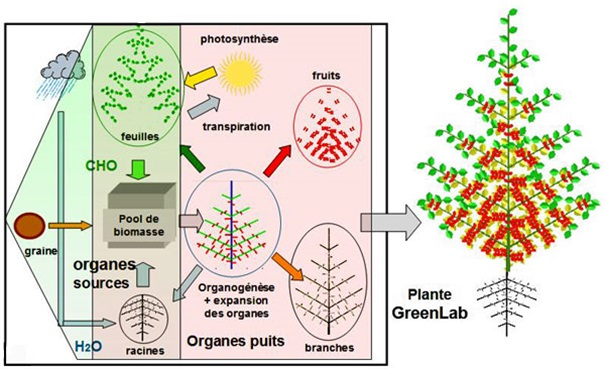
\includegraphics[scale=1]{./img/sGL.jpg}
  \caption{Schéma type d'un modèle GreenLab.}
  \label{fig:schemaGL}
  \end{center}
\end{figure}

Le modèle GreenLab propose une alternative. Il reprend des simplifications utiles du modèle agronome au niveau de la production : la prise en compte de l’architecture individuelle de la plante n’est pas utile au niveau d’un champ, on considère plutôt la distribution des différents types d'organes (densité de feuilles..). Autrement dit, les aspects géométriques peuvent être négligés mais pas la composition quantitative des structures. On fait alors l’hypothèse d’un \emph{pool de biomasse} commun dans lequel les organes vont piocher, et on ne considère que la photosynthèse nette, ie les proportions de glucides qui servent effectivement à la construction de matière sèche des organes. 

Au niveau de l’allocation, cette approche décrit précisément des compartiments d’organes se comportant de façon similaire, ce qui rend l’allocation de biomasse plus facile à modéliser entre organes sources et organes puits et permet de se passer d’une description géométrique ou même topologique exhaustive. Les organes sont générés par cohortes (groupes générés en même temps) de même type grâce à des équations de production des méristèmes selon leur âge physiologique, et des lois de probabilités qui déterminent la croissance, la sénescence et le branching. Et comme tous les organes d’une même cohorte d’organe du même type ont le même état, on peut opérer facilement une factorisation en sous-structures qui rend les calculs plus léger, ainsi le temps de calcul n’est plus proportionnel au nombre d’organe mais seulement à l’âge de la plante. En particulier en multipliant le nombre d’organe de chaque cohorte par la force de puit correspondante et en additionnant le tout on obtient la demande de la plante.

Ensuite l’augmentation $\delta q$ de biomasse de chaque organe est obtenu avec la formule suivante :

\[ \delta q = \phi \cdot Q/D \]

Avec $\phi$ la force de puit, Q la pool de biomasse global et D la demande totale de la plante.

La masse des organes est la somme cumulée de l’augmentation des biomasses, on peut donc obtenir rapidement les dimensions (longueur, diamètre, surface) des organes en utilisant de simples lois géométriques (beaucoup plus simple que celles utilisées lorsque la géométrie est prise en compte dans la production). 

Puis pour que le cycle se répète, la biomasse des compartiments s’obtient  en sommant les cohortes de même organes, en particulier on peut obtenir la masse du feuillage puis la surface foliaire ce qui permettra de déterminer la production de biomasse au prochain cycle. La boucle est bouclée.

Pour résumer, ce modèle est un modèle dynamique de croisance des plantes qui marche par rétroaction entre croissance (production de biomasse) et développement (allocation quantitative et architecture). Le calcul de la production ne prend que peu en compte l’architecture de la plante mais seulement l’équation global de production et les relations sources-puits, ce qui permet des économies de calcul intéressantes et n’empêche pas dans un second temps de générer des structures géométriques fidèles issus d’un modèle de production simplifié mais robuste. Ainsi la plasticité des plantes est très bien représenté par ce modèle et on peut rendre compte de différents phénotypes d’une même espèce dans deux environnement très différents.

\begin{figure}[h]
	\begin{center}
  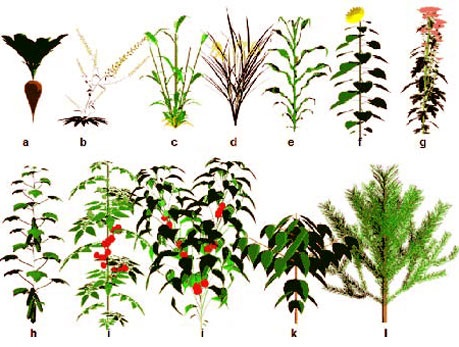
\includegraphics[scale=1]{./img/exempleGL1.jpg}
  \caption{Exemple de plantes générées grâce à GreenLab.}
  \label{fig:exempleGL1}
  \end{center}
\end{figure}

Cela permet notamment la visualisation en images de synthèse très fidèles et complexes de plantes dont la croissance a été modélisé sans prendre en compte le détail géométrique de cette même structure, donc avec un temps de calcul très intéressant. L’augmentation de biomasse de chaque organe a déjà été simplement déterminée grâce aux équations précédentes, dont on déduit également la forme et le volume, de simples règles géométriques positionnent ces organes dans l’architecture selon l’empilement des entre-nœuds autour d’un axe, la phyllotaxie, l’angle de branchement, la courbure des axes, comme on peut le visualiser en Figure~\ref{fig:exempleGL1}.

Comme montré dans la Figure~\ref{fig:exempleP2},
on peut même simuler des paysages entiers grâce à ces méthodes, 
avec le raffinement des paysages fonctionnels qui prennent en compte
raffinement les interactions plantes-environnement, la distribution des
ressources hydriques et des radiations lumineuses entre plantes 
qui sont en compétition.

\begin{figure}[h]
	\begin{center}
	
	
  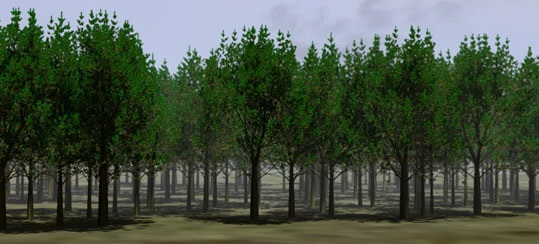
\includegraphics[scale=1.3]{./img/exempleP2.jpg}
  \caption{Paysage fonctionnel généré grâce à GreenLab}
  \label{fig:exempleP2}
  
  \end{center}
\end{figure}
<<<<<<< HEAD
\section{Article modèle LNAS wheat}
\label{ann:articlePierre}}
Le modèle se trouve dans les pages qui suivent.
=======
\newpage
\section{Planning}
\label{ann:planning}

\begin{figure}[H]
  \includegraphics[scale=0.51]{./img/planning.png}
  \caption{Planning de l'organisation des travaux au cours du semestre.}
  \label{fig:planning}
\end{figure}
<<<<<<< HEAD
=======

>>>>>>> origin/master
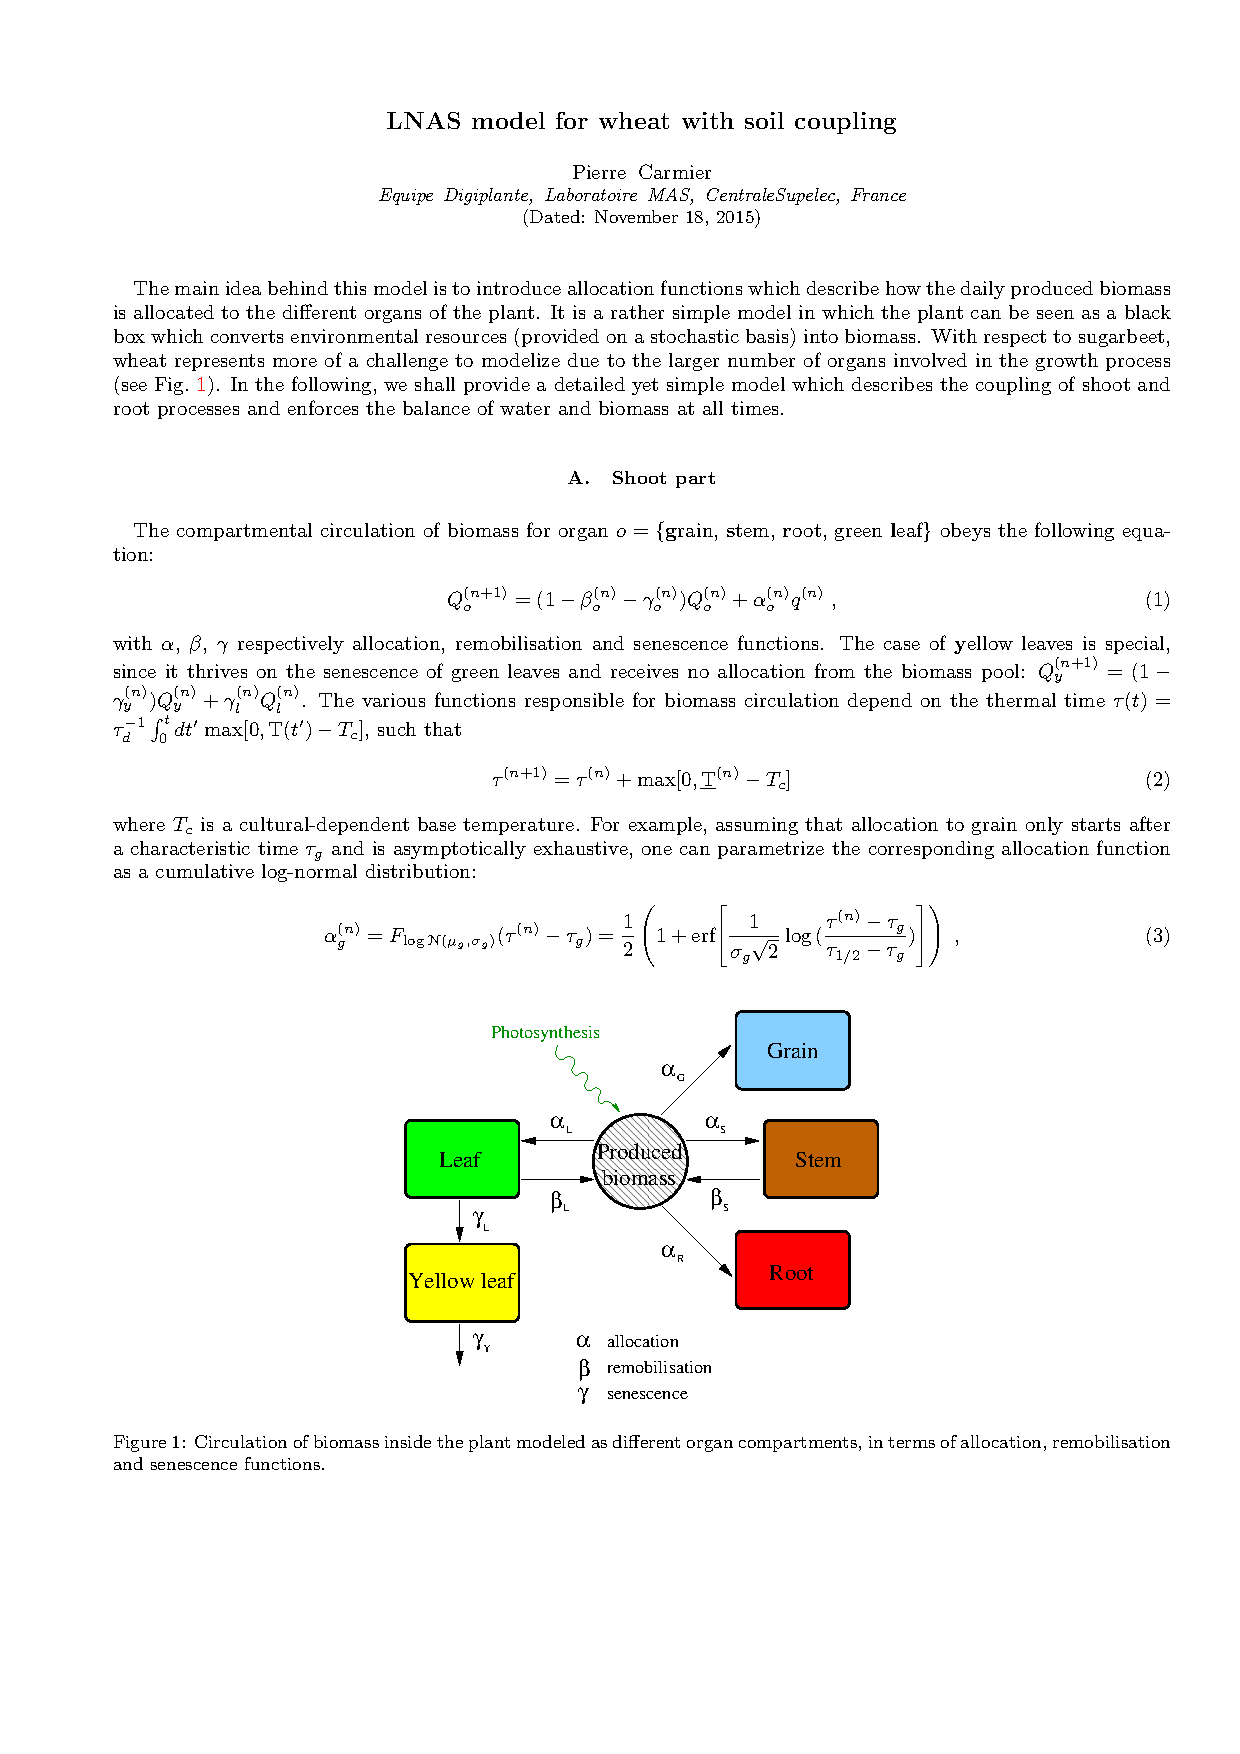
\includepdf[pages=1-3]{./img/LNAS_wheat.pdf}
>>>>>>> 19cad2a8e6509edf5e368d56165ca8dffb5bcb86


\newpage 


\end{document}